% Anonymous manuscript for Neural Computing and Applications.
% The class file is the unmodified Springer Nature sn-jnl template distributed
% with this repository under article/templates.
\documentclass[sn-mathphys-num,Numbered]{sn-jnl}

\usepackage{amsmath,amssymb,bm}
\usepackage{booktabs}
\usepackage{multirow}
\usepackage{tabularx}
\usepackage{graphicx}
\usepackage{hyperref}
\hypersetup{hypertexnames=false}
\usepackage{placeins}
\usepackage{float}
\usepackage{comment}
\usepackage{tikz}
\usetikzlibrary{arrows.meta,positioning,calc}
\newcolumntype{L}{>{\raggedright\arraybackslash}X}
\newcolumntype{C}{>{\centering\arraybackslash}X}
% Shared Springer-compatible table typography; local exceptions should be rare.
\newcommand{\manuscripttablestyle}{\small\setlength{\tabcolsep}{4.5pt}\renewcommand{\arraystretch}{1.10}}

\renewcommand{\topfraction}{0.95}
\renewcommand{\bottomfraction}{0.85}
\renewcommand{\textfraction}{0.05}
\renewcommand{\floatpagefraction}{0.75}

\begin{document}

\title[Metaheuristic optimization for intraday trend classification]{Metaheuristic Hyperparameter Optimization for Intraday Financial Trend Classification: A Benchmark Across Classifier Backbones}

\abstract{Intraday trend classification in futures markets is vulnerable to non-stationarity, weak signal-to-noise ratios, and temporal leakage. A conference precursor used randomized cross-validation and a single optimizer. We extend that work with an auditable benchmark on 15,057 five-minute B3 Mini-Index futures bars and a fixed seven-feature representation inherited from the precursor. Five search methods (RS, GA, PSO, DE, and GWO) tune four classifier backbones (RF, SVM, MLP, and 1D-CNN) under a common 1,000-evaluation budget. A chronological 60/20/20 partition supports two primary holdout protocols: MCC/$F_1$ fitness and weighted training/validation accuracy fitness. A separate exploratory experiment uses three-fold temporal cross-validation with the weighted-accuracy objective. The common chronological test block is scored after selection, with three seeds available per model--optimizer cell; three one-row target alignments cross split boundaries, limiting strict test isolation. We report objective calls and uncached candidate-model fits required to reach 95\% of each run's attained validation-fitness gain. RF leads the MCC/$F_1$ holdout aggregates, whereas MLP has the highest observed accuracy under weighted-accuracy holdout and temporal cross-validation. These comparisons are descriptive; matched-block inference is conditional on the single chronological test interval. Accuracy and MCC are displayed separately, and the cross-validation experiment is not pooled with holdout evidence.}

\keywords{Financial time series $\cdot$ Metaheuristic optimization $\cdot$ Hyperparameter tuning $\cdot$ Matthews correlation coefficient $\cdot$ Temporal validation $\cdot$ Intraday futures}

\maketitle

% ============================================================
% Section 1: Introduction
% Structure follows CARS 5-Move model (NCA_WRITING_DNA.md)
% Citation policy: Prioritizes Neural Computing and Applications (NCA) literature
% ============================================================

\section{Introduction}\label{sec:introduction}

% --- Move 1: Territory (Domain motivation, market specifics, challenges) ---


Financial time-series forecasting remains a challenging computational problem because market data exhibit non-stationarity, nonlinear dependence, structural changes, and substantial noise \cite{jesus2025tda, makridakis2018statistical}. These characteristics become particularly relevant in short-horizon trading, where predictive relationships may weaken or change as market conditions evolve. Among traded financial instruments, futures contracts provide an important setting for this problem because they are widely used for both risk hedging and speculative exposure \cite{jarrow1981forward, souza2025iccsa}. In Brazil, the Mini-Index futures contract (symbol: WIN), traded on Brasil Bolsa Balc\~{a}o (B3) and referenced to the Ibovespa index, is highly liquid and extensively used in intraday operations, making it a relevant environment for computational financial research \cite{souza2024dataset, cardoso2022bovdb}. Predicting directional movements in such markets is therefore scientifically demanding and requires methods capable of extracting useful information from noisy and temporally evolving observations.

% --- Move 2: Model & Search Space (ML models, features, feature selection) ---
Traditional financial forecasting has relied on statistical models such as autoregressive integrated moving average (ARIMA) techniques \cite{box2015time}. As finance and computer science increasingly converged under the computational intelligence paradigm \cite{jiang2021applications}, machine-learning models became widely investigated for financial prediction and classification. Supervised approaches---including Random Forests (RF) \cite{nabipour2020predicting}, Support Vector Machines (SVM) \cite{naik2019optimal}, Multilayer Perceptrons (MLP) \cite{ecer2020mlp_ga_pso}, and 1D Convolutional Neural Networks (1D-CNN) \cite{bandgar2025finchronos}---can capture nonlinear relationships between market variables and future price movements. These models are commonly supplied with technical indicators derived from price, volume, momentum, and volatility. However, large indicator sets may introduce redundant or weakly informative variables, increasing model complexity and potentially degrading generalization \cite{singh2022feature, lei2012feature}. Feature-selection techniques therefore provide an important mechanism for identifying compact and informative predictor subsets \cite{kumar2014feature, souza2025iccsa}.

% --- Move 3: Optimization Paradigm (Hyperparameter tuning, MOAs) ---
Beyond feature selection, predictive performance also depends strongly on hyperparameter configuration \cite{jovanovic2024wann}. Neural and machine-learning models contain structural, regularization, and training parameters that jointly define mixed discrete--continuous and often non-convex search spaces. Gradient-based learning algorithms optimize model parameters once an architecture is defined, but they do not directly solve this outer hyperparameter-search problem when discrete and non-differentiable choices are involved \cite{rajwar2023exhaustive_review}. Metaheuristic Optimization Algorithms (MOAs) provide an alternative by exploring candidate configurations through stochastic search. Evolutionary approaches such as Genetic Algorithms (GA) \cite{goldberg1989ga} and Differential Evolution (DE) \cite{storn1997de}, together with swarm-based methods such as Particle Swarm Optimization (PSO) \cite{kennedy1995pso} and Grey Wolf Optimizer (GWO) \cite{faris2018gwo_review}, have consequently been applied to automated model tuning across neural computing problems \cite{al_bannoud2026accelerating, bashir2026evobagnet}.

% --- Move 4: Literature Gap (3 methodological limitations) ---
Despite the increasing use of metaheuristic optimization in predictive modelling, comparisons between algorithms remain strongly influenced by experimental design. Three methodological limitations are particularly relevant in financial time-series applications:

\begin{enumerate}
    \item \textbf{Unequal computational budgets}: Metaheuristics are commonly expressed using different units such as generations, iterations, populations, particles, or wolves. As a result, apparently similar experimental configurations may correspond to substantially different numbers of objective-function evaluations. Without a common evaluation budget, observed differences may reflect unequal search opportunities rather than differences in optimizer behaviour.

    \item \textbf{Temporal data leakage}: Randomized data partitioning and conventional shuffled cross-validation can violate the chronological structure of financial observations \cite{makridakis2018statistical}. When future observations contribute directly or indirectly to model selection, validation results may provide an overly optimistic estimate of out-of-sample generalization.

    \item \textbf{Dependence on the optimization objective}: Hyperparameter-search outcomes depend not only on the optimizer but also on the metric used to rank candidate configurations. Accuracy alone may provide an incomplete assessment of classification quality, particularly when prediction errors or class distributions are unbalanced \cite{chicco2020mcc}. Moreover, improvements in predictive metrics do not necessarily translate into economically useful trading behaviour once transaction costs and signal frequency are considered.
\end{enumerate}

% --- Move 5: Solution, Framework & Contributions ---
To address these limitations, this paper presents a controlled multi-optimizer benchmark for intraday trend classification using 5-minute B3 Mini-Index futures data. A compact seven-indicator subset previously identified through Information Gain is used as a fixed input representation, while five optimization strategies---Random Search (RS), Genetic Algorithm (GA), Particle Swarm Optimization (PSO), Differential Evolution (DE), and Grey Wolf Optimizer (GWO)---are evaluated across four classifier families: MLP, SVM, RF, and 1D-CNN. All optimizers operate under the same objective-function evaluation budget of $N_{\mathrm{eval}} = 1{,}000$ evaluations per seed, and temporal ordering is preserved through chronological model selection followed by scoring on a nominally subsequent test block. Because three one-row-shifted target labels cross partition boundaries, strict test isolation is not achieved at those rows. The study further contrasts a compound MCC-driven objective ($0.60\,\mathrm{MCC} + 0.40\,F_1$) with accuracy-based optimization protocols. Predictive performance is complemented by convergence analysis, non-parametric statistical testing, and out-of-sample economic evaluation under transaction costs.

The main contribution of this study is the development of a controlled experimental framework that disentangles the effects of optimizer family, predictive model, validation objective, and computational budget in intraday financial classification. Rather than evaluating metaheuristics under isolated or algorithm-specific settings, the proposed benchmark places five optimization strategies and four predictive model families under the same temporal data partitions, the same feature representation, and an equal number of objective-function evaluations. By combining predictive metrics, convergence behaviour, matched statistical testing, and economic evaluation under transaction costs, the study provides a more complete assessment of optimizer robustness and practical relevance. In this sense, the proposed framework extends existing approaches to intraday futures classification by integrating feature selection, multiple optimization strategies, temporal validation, and equal computational budgets within a unified and reproducible comparative methodology.

% --- Move 6: Outline ---
The remainder of this manuscript is organized as follows. Section~\ref{sec:literature_review} presents the related literature and establishes the research gap. Section~\ref{sec:methods} describes the dataset, feature selection, predictive models, optimization algorithms, search spaces, and experimental protocol. Section~\ref{sec:results} reports the predictive results, convergence behaviour, statistical analyses, and economic evaluation. Section~\ref{sec:discussion} discusses the findings, methodological implications, and limitations. Finally, Section~\ref{sec:conclusion} summarizes the main conclusions and outlines future research directions.
% ============================================================
% Section 2: Related Work and Literature Positioning
% Structured literature search and narrative synthesis; this is not presented as a PRISMA systematic review.
% ============================================================

\section{Related Work and Literature Positioning}\label{sec:literature_review}

The intersection of computational intelligence, metaheuristic optimization, and financial time-series forecasting has generated an extensive body of literature over the past decade \cite{henrique2019stock_review, rajwar2023exhaustive_review, jiang2021applications}. Comprehensive surveys have categorized machine learning applications in financial prediction \cite{henrique2019stock_review, jiang2021applications}, systematically reviewed metaheuristic search paradigms such as Particle Swarm Optimization \cite{gad2022pso_comprehensive, wang2018pso_comprehensive} and Grey Wolf Optimizer \cite{faris2018gwo_review}, and benchmarked neural forecasting architectures under computational constraints \cite{dhingra2025solar, jovanovic2024wann}. However, despite substantial published progress in premier neural computing journals \cite{billah2024nca_moving_average, bandgar2025finchronos, al_bannoud2026accelerating, bashir2026evobagnet}, existing reviews and empirical benchmarks have not systematically evaluated the interaction between equal-budget metaheuristic tuning, temporal validation integrity, and out-of-sample trading performance. We use a structured search and narrative synthesis to position the benchmark across feature selection, model backbones, metaheuristic search, and validation protocols, and to identify methodological gaps relevant to this study.

\subsection{Search Scope and Research Questions}\label{subsec:selection_protocol}

Relevant literature was identified through a structured search of major scholarly databases: IEEE Xplore, Scopus, Web of Science, and SpringerLink (specifically targeting \textit{Neural Computing and Applications}). The search was executed using the following structured Boolean query:
\begin{itemize}
    \item (\texttt{"metaheuristic"} OR \texttt{"genetic algorithm"} OR \texttt{"particle swarm"} OR \texttt{"grey wolf"})
    \item AND (\texttt{"feature selection"} OR \texttt{"technical indicators"} OR \texttt{"Information Gain"})
    \item AND (\texttt{"futures market"} OR \texttt{"intraday forecasting"} OR \texttt{"trend classification"})
\end{itemize}

The review was bounded to peer-reviewed journal articles and top-tier conference proceedings published between 2019 and 2026. Candidate studies were screened against explicit eligibility criteria:
\begin{itemize}
    \item \textbf{Inclusion Criteria}: (i) evaluation of automated feature selection or metaheuristic hyperparameter tuning on financial or complex time-series classification/forecasting; (ii) explicit disclosure of validation protocols and search space boundaries; and (iii) reporting of empirical predictive or out-of-sample financial metrics.
    \item \textbf{Exclusion Criteria}: Studies lacking reproducible experimental parameters, omitting candidate evaluation budget details, or failing to disclose optimization constraints were excluded.
\end{itemize}

The synthesis discusses 15 representative studies in Table~\ref{tab:literature_gap}. The benchmark is organized around three research questions (RQs):
\begin{enumerate}
    \item \textbf{RQ1 (Budget Parity)}: How do stochastic metaheuristic search operators (RS, GA, PSO, DE, GWO) compare across distinct classifier backbones (RF, SVM, MLP, 1D-CNN) when restricted to a strictly equal candidate evaluation budget cap ($N_{\mathrm{eval}} = 1{,}000$)?
    \item \textbf{RQ2 (Chronological evaluation)}: How do the evaluated backbones and selection protocols perform on a common chronologically subsequent test interval when model selection preserves temporal ordering?
    \item \textbf{RQ3 (Predictive and economic outcomes)}: How do predictive outcomes under the evaluated selection protocols relate to results from the study’s fixed-cost next-bar trading calculation?
\end{enumerate}




\FloatBarrier

\subsection{Classifier Backbones and Input Representations}\label{subsec:backbones_features}

The quality and information density of the input representation are central determinants of supervised intraday trend prediction \cite{singh2022feature}. Open, high, low, close, and volume observations encode the market state, but short-horizon bars are also affected by microstructural noise, regime shifts, and high variance. For this reason, financial machine-learning studies commonly transform raw bar data into technical descriptors representing complementary aspects of price behaviour: momentum, trend, dispersion, and volatility \cite{billah2024nca_moving_average, hunter1986exponentially, bollinger1992using}. Such representations do not create information; rather, they provide a structured hypothesis space through which a learner can test whether recent price and volume dynamics carry directional content.

The expansion of the indicator set must nevertheless be controlled. Indicators derived from common prices and overlapping lookback windows are often strongly correlated, so a large technical library can amplify redundancy, increase estimation variance, and make model ranking sensitive to incidental patterns in the development sample \cite{lei2012feature, kumar2014feature}. Feature selection is therefore a component of model design rather than a preliminary convenience: it reduces the dimensionality exposed to subsequent learning and hyperparameter search, while retaining descriptors with a demonstrable association with the target. Information Gain (IG) is a transparent filter criterion for this purpose, ranking candidate indicators by their reduction of class uncertainty \cite{lei2012feature, anonymous2025precursor}. Although a univariate ranking does not guarantee an optimal multivariate subset, its low computational cost and auditability make it appropriate for constructing a compact technical representation. The mathematical formulation and empirical application of IG in the present benchmark are detailed in Section~\ref{sec:featureselection}.

The literature spans several classifier families whose distinct inductive biases make a single preferred backbone unlikely across all market representations:
\begin{itemize}
    \item \textbf{Ensemble decision trees}, represented by Random Forest (RF), aggregate decorrelated trees built from bootstrap samples and randomly selected feature subsets. Their partition-based structure accommodates non-linear interactions and can be relatively robust to noisy descriptors \cite{nabipour2020predicting}.
    \item \textbf{Kernel margin classifiers}, represented by Support Vector Machines (SVM), seek separating hyperplanes with a maximum-margin principle. Kernel mappings, including the radial-basis-function kernel, permit non-linear decision surfaces while retaining a well-defined optimization objective \cite{naik2019optimal}.
    \item \textbf{Feedforward neural networks}, represented by Multilayer Perceptrons (MLP), learn non-linear mappings through stacked fully connected layers and backpropagation. Their expressive capacity is accompanied by sensitivity to architectural and regularization choices \cite{ecer2020mlp_ga_pso}.
    \item \textbf{One-dimensional convolutional neural networks} (1D-CNN) apply shared local filters to ordered input windows. This construction can capture short-range patterns while using parameter sharing to constrain the number of learned weights \cite{bandgar2025finchronos, dhingra2025solar}.
\end{itemize}

These families therefore represent different hypotheses about how directional information is encoded. Their comparative use is more informative than selecting a single algorithm a priori, particularly because changes in feature representation and hyperparameterization can alter the observed ranking of classifiers \cite{nabipour2020predicting, mutinda2026hybrid}. The specific representations, search domains, and fitted architectures adopted in this study are defined in Section~\ref{sec:methods}.

\subsection{Metaheuristic Optimization Paradigms}\label{subsec:metaheuristic_paradigms}

Hyperparameter selection is naturally formulated as a black-box optimization problem. Let $\boldsymbol{\theta} \in \Omega$ denote a feasible model configuration, where $\Omega$ can contain continuous, integer, categorical, and conditional variables. A validation criterion $f(\boldsymbol{\theta})$ is obtained only after fitting and evaluating the corresponding learning pipeline, and the search objective is
\begin{equation}\label{eq:metaheuristic_objective}
\boldsymbol{\theta}^{\star} = \underset{\boldsymbol{\theta} \in \Omega}{\operatorname{arg\,max}}\; f(\boldsymbol{\theta}).
\end{equation}
Unlike weight training, this objective need not be differentiable with respect to $\boldsymbol{\theta}$. Tree depth, number of hidden units, kernel choices, and regularization settings may also be discrete or conditionally active. Population-based metaheuristics are consequently attractive because they navigate such mixed spaces without gradient information and can balance broad exploration against local refinement \cite{jovanovic2024wann, faris2018gwo_review, rajwar2023exhaustive_review}.

In this context, a “candidate evaluation” should mean one complete configuration assessment under an unchanged validation protocol. This distinction is important: iterations and generations are internal counters, whereas the number of evaluated candidates is the common computational unit through which heterogeneous search procedures can be compared.

Figure~\ref{fig:backbone_optimizer_taxonomy} provides a compact taxonomy of the learning and search families considered in this literature. It distinguishes the classifier hypothesis spaces from the mechanisms used to select their configurations, while retaining the shared objective of validation-based model selection.

\begin{figure}[htbp]
\centering

\resizebox{0.96\linewidth}{!}{%
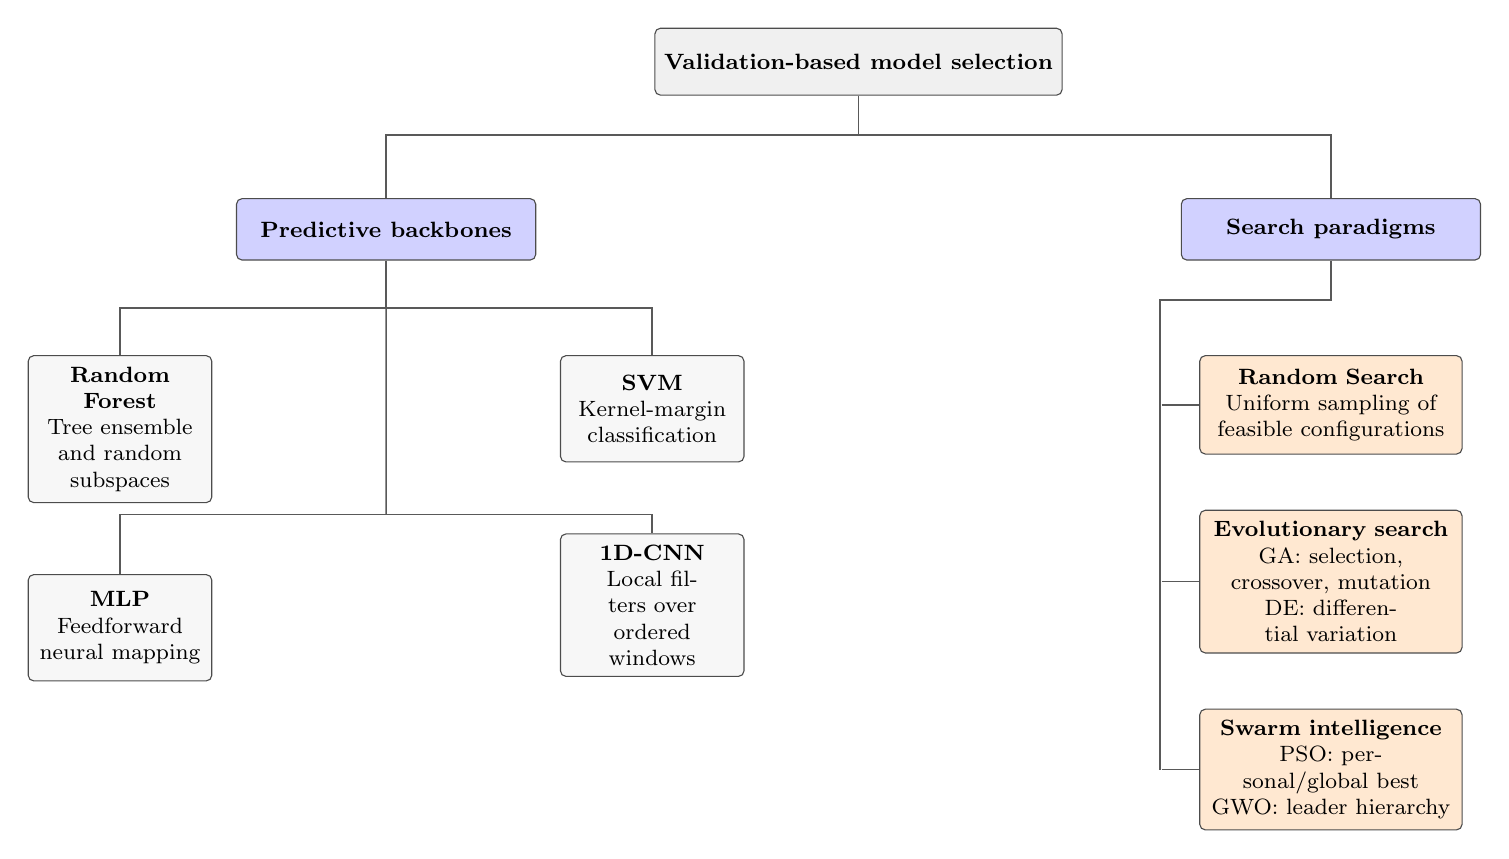
\begin{tikzpicture}[
    node distance=8mm and 10mm,
    every node/.style={
        font=\footnotesize,
        align=center
    },
    root/.style={
        draw=black!70,
        fill=black!6,
        rounded corners=2pt,
        minimum width=4.8cm,
        minimum height=0.85cm,
        font=\bfseries\footnotesize
    },
    family/.style={
        draw=black!70,
        fill=blue!18,
        rounded corners=2pt,
        minimum width=3.8cm,
        minimum height=0.78cm,
        font=\bfseries\footnotesize
    },
    classifier/.style={
        draw=black!70,
        fill=black!3,
        rounded corners=2pt,
        text width=2.05cm,
        minimum height=1.35cm,
        inner sep=4pt
    },
    search/.style={
        draw=black!70,
        fill=orange!18,
        rounded corners=2pt,
        text width=3.05cm,
        minimum height=1.25cm,
        inner sep=4pt
    },
    connector/.style={
        draw=black!65,
        line width=0.55pt
    }
]

% ============================================================
% Root
% ============================================================

\node[root] (root)
{Validation-based model selection};

% ============================================================
% Main families
% ============================================================

\node[family, below left=13mm and 15mm of root]
(backbones)
{Predictive backbones};

\node[family, below right=13mm and 15mm of root]
(searchfam)
{Search paradigms};

% Root branch
\coordinate (rootjunction) at ($(root.south)+(0,-5mm)$);

\draw[connector]
(root.south) -- (rootjunction);

\draw[connector]
(backbones.north) |- (rootjunction);

\draw[connector]
(searchfam.north) |- (rootjunction);

% ============================================================
% Predictive backbones
% ============================================================

\node[classifier, below left=12mm and 3mm of backbones]
(rf)
{\textbf{Random Forest}\\
Tree ensemble\\
and random subspaces};

\node[classifier, below right=12mm and 3mm of backbones]
(svm)
{\textbf{SVM}\\
Kernel-margin\\
classification};

\node[classifier, below=9mm of rf]
(mlp)
{\textbf{MLP}\\
Feedforward\\
neural mapping};

\node[classifier, below=9mm of svm]
(cnn)
{\textbf{1D-CNN}\\
Local filters over\\
ordered windows};

% Central backbone structure
\coordinate (backboneTop)
    at ($(backbones.south)+(0,-6mm)$);

\coordinate (backboneBottom)
    at ($(mlp.north)!0.5!(cnn.north)+(0,5mm)$);

\draw[connector]
(backbones.south) -- (backboneTop);

\draw[connector]
(backboneTop) -- (backboneBottom);

\draw[connector]
(rf.north) |- (backboneTop);

\draw[connector]
(svm.north) |- (backboneTop);

\draw[connector]
(mlp.north) |- (backboneBottom);

\draw[connector]
(cnn.north) |- (backboneBottom);

% ============================================================
% Search paradigms
% ============================================================

\node[search, below=12mm of searchfam]
(rs)
{\textbf{Random Search}\\
Uniform sampling of\\
feasible configurations};

\node[search, below=7mm of rs]
(evo)
{\textbf{Evolutionary search}\\
GA: selection, crossover, mutation\\
DE: differential variation};

\node[search, below=7mm of evo]
(swarm)
{\textbf{Swarm intelligence}\\
PSO: personal/global best\\
GWO: leader hierarchy};

% Vertical search spine
\coordinate (searchTop)
    at ($(searchfam.south)+(-2.15cm,-5mm)$);

\coordinate (searchBottom)
    at ($(swarm.west)+(-5mm,0)$);

\draw[connector]
(searchfam.south)
-- ++(0,-5mm)
-| (searchTop);

\draw[connector]
(searchTop)
-- (searchBottom |- searchTop)
-- (searchBottom);

\draw[connector]
(searchTop |- rs.west) -- (rs.west);

\draw[connector]
(searchTop |- evo.west) -- (evo.west);

\draw[connector]
(searchTop |- swarm.west) -- (swarm.west);

\end{tikzpicture}%
}

\caption{
Conceptual taxonomy linking predictive backbones with
hyperparameter-search strategies in the reviewed literature.
The left branch denotes alternative classifier hypothesis spaces,
whereas the right branch distinguishes unguided sampling,
evolutionary search, and swarm intelligence.
The precise search domains and experimental controls are
specified in Section~\ref{sec:methods}.
}
\label{fig:backbone_optimizer_taxonomy}

\end{figure}

Evolutionary algorithms maintain a population of candidate configurations and improve it through selection and variation. Genetic Algorithms (GA) emulate selection, crossover, and mutation: configurations with stronger fitness are preferentially retained or recombined, while mutation introduces new material into the population \cite{goldberg1989ga, jovanovic2024wann}. This representation-agnostic cycle is well suited to mixed hyperparameter spaces after appropriate encoding and constraint handling.

Differential Evolution (DE) is also population based, but creates candidate displacements from scaled differences between population members. A canonical donor-vector form is
\begin{equation}\label{eq:de_mutation}
\mathbf{v}_{i}^{t} = \mathbf{x}_{r_1}^{t} + F\left(\mathbf{x}_{r_2}^{t} - \mathbf{x}_{r_3}^{t}\right),
\end{equation}
where $r_1$, $r_2$, and $r_3$ index distinct population members and $F$ scales the differential displacement. Crossover then combines the donor with a target vector, and selection retains the better candidate \cite{storn1997de}. The use of population differences gives DE a self-adaptive search scale, although its practical behaviour still depends on encoding, bounds, and the chosen mutation and crossover strategy.

Swarm methods update candidates by combining individual experience with population-level information. In Particle Swarm Optimization (PSO), each particle has a position $\mathbf{x}_{i}^{t}$, a velocity $\mathbf{v}_{i}^{t}$, a personal best position $\mathbf{p}_{i}^{t}$, and an incumbent swarm-best position $\mathbf{g}^{t}$. Its standard update is
\begin{align}
\mathbf{v}_{i}^{t+1} &= \omega\mathbf{v}_{i}^{t} + c_{1}r_{1}\left(\mathbf{p}_{i}^{t}-\mathbf{x}_{i}^{t}\right) + c_{2}r_{2}\left(\mathbf{g}^{t}-\mathbf{x}_{i}^{t}\right), \label{eq:pso_velocity}\\
\mathbf{x}_{i}^{t+1} &= \mathbf{x}_{i}^{t} + \mathbf{v}_{i}^{t+1}, \label{eq:pso_position}
\end{align}
where $\omega$ controls inertia, $c_{1}$ and $c_{2}$ weight cognitive and social attraction, and $r_{1},r_{2}$ are random variates. This formulation makes the exploration--exploitation trade-off explicit and is the foundation for the broad family of PSO variants reviewed by Gad \cite{kennedy1995pso, gad2022pso_comprehensive}.

Grey Wolf Optimizer (GWO) uses a different collective metaphor. Candidate solutions are ranked into leading $\alpha$, $\beta$, and $\delta$ wolves, while the remaining wolves update their positions by encircling and approaching these leaders. Its control schedule progressively shifts the search from exploration to exploitation \cite{faris2018gwo_review, al_bannoud2026accelerating}. Despite distinct metaphors, PSO and GWO share the same benchmarking requirement: each update must be translated into feasible configurations and assessed under the same validation rule.

Random Search (RS) is an indispensable baseline because it samples feasible configurations without an adaptive search trajectory. It establishes whether the additional mechanisms of evolutionary or swarm search improve solution quality beyond unguided sampling from the same search space \cite{bergstra2012random_search}. A credible comparison must therefore control the parameter domain, candidate-evaluation count, validation data, random replication, and reporting metrics. Equalizing only the nominal number of generations or iterations is insufficient when algorithms evaluate different numbers of candidates per update.

The comparative evidence also highlights recurring weaknesses: unequal computational budgets can confound search quality with search effort; randomized validation can compromise temporal integrity; and classification-only reporting may not establish economic value after transaction costs \cite{ecer2020mlp_ga_pso, bandgar2025finchronos, billah2024nca_moving_average}. These issues are synthesized in Section~\ref{subsec:comparative_synthesis}; the concrete controls used by the present benchmark are specified only in Section~\ref{sec:methods}.


\subsection{Comparative Synthesis of Representative Studies}\label{subsec:comparative_synthesis}

To establish the state of the art and pinpoint persistent methodological gaps, Table~\ref{tab:literature_gap} synthesizes 15 representative published studies from 2019 to 2026 alongside the present benchmark work. Studies are evaluated across six technical dimensions: Study \& Year, Application Domain \& Data, Model Backbones, Optimization \& Feature Paradigms, Validation Protocol, and Identified Methodological Gap.

\begin{table}[!htbp]
\caption{Structured literature comparison matrix auditing representative studies in financial machine learning, metaheuristic hyperparameter tuning, and temporal validation protocols against identified methodological gaps.}
\label{tab:literature_gap}
\centering
\manuscripttablestyle
% Footnotesize is retained for this dense full-width synthesis matrix.
\footnotesize
\begin{tabularx}{\linewidth}{@{}>{\raggedright\arraybackslash}p{0.18\linewidth} >{\raggedright\arraybackslash}p{0.22\linewidth} >{\raggedright\arraybackslash}p{0.29\linewidth} >{\raggedright\arraybackslash}X@{}}
\toprule
Study \& Year & Domain and models & Optimization, features, and validation & Primary methodological gap \\
\midrule
Nabipour et al.\ (2020) \cite{nabipour2020predicting} & Stock-index trend; RF, SVM, ANN, XGBoost & Technical indicators; train/test split & No metaheuristic hyperparameter tuning. \\
Jovanovic et al.\ (2024) \cite{jovanovic2024wann} & Crop yield; weight-agnostic neural networks & Metaheuristic tuning; train/test & Non-financial domain; no equal-budget financial benchmark. \\
Naik \& Mohan (2019) \cite{naik2019optimal} & NSE equities; ANN classifier & Boruta feature selection; train/test & Static parameters; no metaheuristics. \\
Ecer et al.\ (2020) \cite{ecer2020mlp_ga_pso} & Financial trend; MLP & GA and PSO tuning; $K$-fold CV & Unconstrained budget; single classifier. \\
Billah et al.\ (2024) \cite{billah2024nca_moving_average} & Intraday equities; heuristic models & Moving-average rules; standard split & No neural hyperparameter tuning. \\
Bareket \& P{\^a}rv (2024) \cite{bareket2024adaptive} & Surge detection; adaptive ML & Technical indicators; medium-term split & Evaluation restricted to static features. \\
Bandgar et al.\ (2025) \cite{bandgar2025finchronos} & Financial forecasting; ensembles & Default tuning; random split & No evaluation budget cap; temporal leakage risk. \\
Rahim et al.\ (2025) \cite{rahim2025technical} & 5-min futures; single neural model & Single GA; train/test split & Single GA; no multi-optimizer benchmark. \\
Dhingra et al.\ (2025) \cite{dhingra2025solar} & Solar PV; LSTM, CNN-LSTM & RAdam, Lookahead, Adam; sequential split & Non-financial domain; stochastic optimizers omitted. \\
Mutinda \& Yong (2026) \cite{mutinda2026hybrid} & Financial market; ensembles & SEDT feature selection; $K$-fold CV & Feature selection without tuning. \\
Simatupang et al.\ (2026) \cite{simatupang2026stock} & IDX stock index; Bayesian RF & Bayesian optimization; random $K$-fold CV & Random CV risks temporal information leakage. \\
Al Bannoud et al.\ (2026) \cite{al_bannoud2026accelerating} & Kinetics series; ANN--ODE surrogate & GWO, PSO, GA, ABC; multi-partition & Non-financial; unconstrained search budget. \\
Bashir et al.\ (2026) \cite{bashir2026evobagnet} & NSE equities; bagging ensemble & (1+1) evolutionary algorithm; train/test & Single EA; no budget cap. \\
\textit{[Anonymized Precursor A]} (2025) \cite{anonymous2025precursor} & Intraday B3 futures; RF & InfoGain + default RF; sequential 60/20/20 & Untuned baseline; no metaheuristics. \\
\textit{[Anonymized Precursor B]} (2026) \cite{anonymous2026precursor} & Intraday B3 futures; MLP, SVM, RF & InfoGain + single GA; 5-fold CV & Single GA; unconstrained generation budget. \\
\textbf{Present Work} & \textbf{Intraday B3 futures; MLP, SVM, RF, 1D-CNN} & \textbf{InfoGain + RS, GA, PSO, DE, GWO; sequential 60/20/20} & \textbf{Equal $N_{\mathrm{eval}}=1{,}000$, 3 seeds, fee backtest.} \\
\botrule
\end{tabularx}
\end{table}
\FloatBarrier

As synthesized in Table~\ref{tab:literature_gap}, three primary methodological flaws permeate the existing literature on metaheuristic financial forecasting:
\begin{enumerate}
    \item \textit{The Budget Inequality Flaw}: Prior studies routinely compare metaheuristics without enforcing a strict candidate evaluation cap ($N_{\mathrm{eval}}$). Because stochastic optimization performance scales with function evaluations, superiority claims in unconstrained studies often reflect unequal computational budgets rather than algorithmic search efficiency \cite{dhingra2025solar, ecer2020mlp_ga_pso}.
    \item \textit{The Temporal Data Leakage Flaw}: Financial machine learning research frequently relies on randomized $K$-fold cross-validation or data shuffling \cite{simatupang2026stock, makridakis2018statistical}. Shuffling sequential intraday price bars allows future market information to contaminate historical training folds, yielding artificially inflated predictive accuracy scores that collapse during live execution.
    \item \textit{The Classification-Economic Disconnect Flaw}: Hyperparameter tuning is overwhelmingly conducted against raw accuracy or cross-entropy loss \cite{chicco2020mcc, anonymous2025precursor}. In high-frequency futures trading, raw accuracy ignores class imbalance and trade execution costs. A classifier achieving high nominal accuracy can incur net financial losses once exchange transaction fees and slippage are deducted.
\end{enumerate}

Figure~\ref{fig:literature_scope_by_year} shows the distribution of the 15 representative studies by publication year and optimizer-comparison scope. 

\begin{figure}[htbp]
\centering
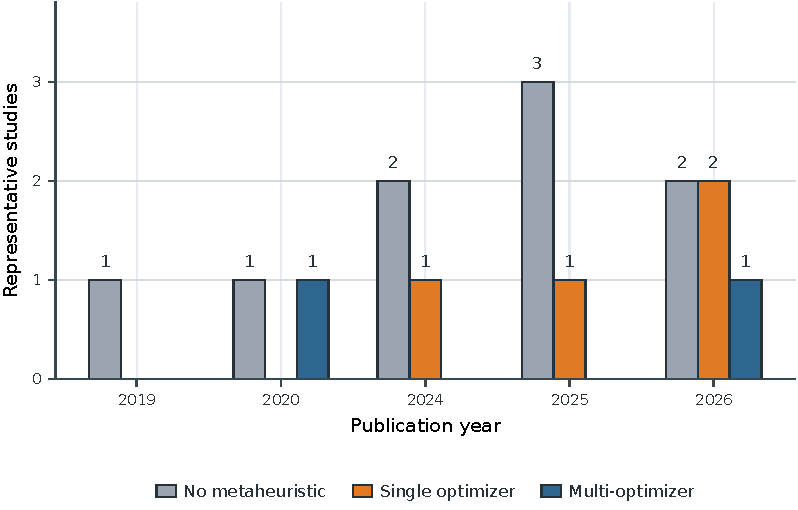
\includegraphics[width=0.90\linewidth]{figures/literature_scope_by_year.pdf}
\caption{Distribution of the 15 representative prior studies included in the literature synthesis, grouped by publication year and the scope of optimizer comparison. A study is assigned to one category according to its primary experimental design; the present work is excluded. The limited number of multi-optimizer studies motivates the controlled benchmark developed in this paper.}
\label{fig:literature_scope_by_year}
\end{figure}

\subsection{Research Positioning and Study Contribution}\label{sec:research_positioning}

The literature synthesis reveals that prior studies have typically addressed only subsets of the experimental problem considered here. Existing financial forecasting research has investigated feature selection, individual predictive models, or isolated metaheuristic tuning strategies, but these components are rarely evaluated simultaneously under common temporal and computational controls. The precursor studies in this research line first established the value of Information Gain feature selection for B3 Mini-Index futures and subsequently explored Genetic Algorithm-based hyperparameter tuning. The present work moves beyond these isolated stages by treating model selection and optimizer behaviour as components of a unified comparative benchmark.

The methodological extension is therefore not limited to increasing the number of models or optimization algorithms. The proposed framework changes the experimental control structure by combining four heterogeneous predictive backbones with five search strategies under a common feature representation, identical temporal partitions, and an equal objective-function evaluation budget. It further evaluates how optimizer behaviour changes under alternative validation objectives and complements predictive metrics with convergence analysis, matched statistical testing, and economic evaluation under transaction costs.

This design allows the study to distinguish performance differences associated with optimizer behaviour from those induced by model architecture, validation objective, or unequal search effort. Accordingly, the contribution is positioned as a controlled and reproducible model--optimizer benchmark for intraday financial classification rather than as an incremental extension of a single metaheuristic method.

\section{Materials and Methods}\label{sec:methods}\label{sec:methodology}

This section presents the methodology adopted in this study. Figure~\ref{fig:workflow} provides an overview of the methodological flow adopted in this study. The diagram highlights each step of the process, illustrating the flow from data acquisition to model optimization and evaluation.

\begin{figure}[ht]
    \centering
    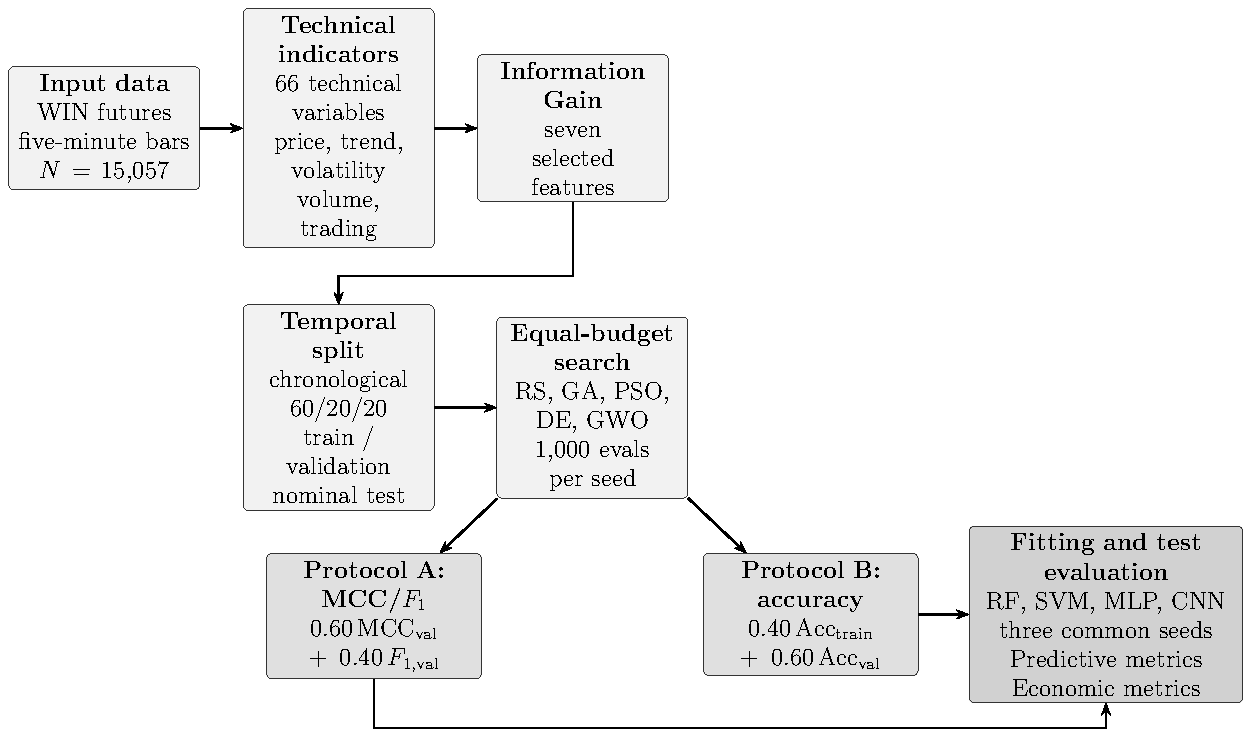
\includegraphics[width=0.90\linewidth]{figures/methodology_workflow_vector.pdf}
    \caption{Overview of the proposed methodology. The benchmark reuses the precursor’s fixed
Information-Gain representation while enforcing a chronological split, equal optimizer budget, and
two separated validation objectives.}
    \label{fig:workflow}
\end{figure}

\subsection{Input Data}
\label{sec:data}

The data used in this study were obtained from BovDbV2 \cite{souza2024dataset}, an extension of the original BovDb \cite{cardoso2022bovdb}. The database provides publicly available and pre-processed B3 market data for research purposes, covering listed assets from 1995 to 2024. BovDbV2 additionally includes intraday observations aggregated into 5-minute intervals for the first half of 2024, enabling the analysis of short-horizon market behaviour.

For the present study, the analysis focuses on Mini Ibovespa Futures (WIN) contracts traded between January and June 2024. The selected contracts correspond to the most actively traded maturities over the analyzed period: WING24 and WINJ24 in January--February, WINJ24 and WINM24 in March--April, and WINM24 and WINQ24 in May--June. After preprocessing and construction of the modelling dataset, the final sample contains 15,057 chronological observations.

The explanatory variables are technical indicators computed from completed five-minute price and volume bars. The binary regime labels (0, downtrend; 1, uptrend) are generated from peak-and-trough structure detected on hourly candles resampled from the five-minute price series. The detector groups consecutive bullish and bearish hourly candles, locates the highest or lowest close within each run, refines that pivot to the corresponding extreme five-minute close, and checks the following hourly interval for a more extreme close. The resulting pivot states are assigned to five-minute observations and carried forward; the initial segment is assigned retrospectively from the first detected pivot. We reproduced this procedure against the archived label database and obtained exact agreement for all 23,181 stored rows. In the modeling dataset, each five-minute feature row is paired with the next retained regime-label row for the same ticker, $y_{i,t} = r_{i,t+1}$. This alignment agrees with the archived label database for all 15,053 rows with a successor, including 196 session-final rows whose successor is in the following session. Four final rows, one per ticker series, have no successor and retain their contemporaneous label. Thus, the benchmark is a next-observation regime-prediction task, with four terminal-row exceptions. Predictions are available after bar $t$ closes; the economically aligned entry is at the open of bar $t+1$. The hourly pivots and their confirmation are retrospective, so this one-bar shift does not make the target itself causal.

All observations are kept in their original chronological order. The first 9,034 observations are assigned to the training set, the following 3,011 observations to the validation set, and the final 3,012 observations to the nominal test set. No random shuffling is performed. Because the target is shifted by one retained row, however, one training observation at the split boundary is paired with a validation-period label, and two validation observations are paired with test-period labels. These three boundary observations were retained in the reported experiments; thus, the test block is chronologically subsequent, but its labels are not fully isolated from model selection. A cutoff audit that reran the recovered label routine using only price history available through each cutoff found no label changes among the other 9,032 training and 3,008 validation targets checked. This audit addresses retrospective changes to the recovered pivot labels, not the three direct one-row crossings or the longer confirmation horizon of the pivot rule. In addition, four final per-ticker rows have no next retained observation and use their contemporaneous source label. Results should therefore be interpreted with these boundary and terminal-row exceptions in mind.

\subsection{Generation of Technical Analysis Indicators}
\label{sec:indicators}

Technical indicators were built from the intraday dataset to capture short-term price changes. Key metrics—Simple Moving Average (SMA), Exponential Moving Average (EMA), and Standard Deviation—were calculated using short time windows (3, 5, 7, and 9 periods) to enhance sensitivity to rapid market shifts, where significant moves can happen in minutes \cite{hunter1986exponentially}.

To capture changes in trend slope and momentum, attributes derived from the differences between calculated moving averages were also constructed. For example, the difference between the 7-period SMA and the 3-period SMA is defined in Eq. (1) as:

\begin{equation}
\text{SMA}_{7-3} = \text{SMA}_{7} - \text{SMA}_{3},
\end{equation}

A central preprocessing step consisted of normalizing the technical indicators \cite{singh2022feature}, as well as the opening and closing prices, in order to place all variables on a common numerical scale. For each 5-minute intraday window, a min–max–type scaling was applied, in which each feature was transformed according to Eq. (2):

\begin{equation}
\text{Feature}_{\text{norm}} = \frac{\text{Feature} - \text{Low}}{\text{High} - \text{Low}}.
\end{equation}

Where \textit{High} and \textit{Low} correspond to the maximum and minimum prices observed within the same 5-minute interval, and \textit{Feature} denotes any technical indicator or price-based variable being normalized. This transformation maps the features predominantly to the interval $[0,1]$, while preserving their relative positions within the intraday price range, thereby reducing the impact of heterogeneous attribute scales and facilitating the learning of machine learning models. This normalization procedure, combined with historical information on open, high, low, average, close, bid, ask, trade volume, and number of shares, results in a total of 66 constructed features.

\subsection{Feature Selection Method}
\label{sec:featureselection}
The predictive pipeline incorporates a structured feature selection stage based on technical analysis indicators. Following the approach proposed in \cite{souza2024dataset}, multiple selection strategies are evaluated to identify the most informative feature subsets, thereby enhancing model discrimination while reducing redundancy and noise inherent in high-dimensional financial data.

In the precursor, feature-selection strategies included filters and wrappers. The Information Gain ranking was produced in WEKA using only the chronological training partition (January--March 2024), separated by the number of five-minute observations in that interval; the April--June test partition was excluded, as confirmed by the researcher. The ranking was then recorded as a fixed list in the Python workflow. Its first seven features form the compact representation used here. The present benchmark applies that inherited mask without re-estimating selection on its own training partition, so its conclusions remain conditional on the selected representation. The original WEKA project/output is not archived, but the selected feature list and the subsequent train/test data split are preserved in the project files.

The selected features, ranked by their Information Gain scores, include the EMA-based differences $5\!-\!3$ and $7\!-\!3$, their normalized counterparts, the normalized 9-period SMA, the $9\!-\!3$ EMA difference, and the normalized 7-period EMA. 

The seven ranked descriptors listed above are used unchanged as the input representation for all four backbones and five optimizers in this benchmark.

\subsection{Implemented Classifier Architectures and Search Spaces}
\label{sec:classifier_architectures}

To benchmark metaheuristic search performance across fundamentally distinct hypothesis spaces, four classifier backbones were implemented: Random Forest (RF), Support Vector Machines (SVM), Multilayer Perceptron (MLP), and 1D Convolutional Neural Networks (1D-CNN). Figure~\ref{fig:classifier_backbones} illustrates the structural decision mechanisms and layer topologies of these four implemented architectures.
For the neural backbones, the MLP has one tanh hidden layer with dropout and a sigmoid output; the implementation uses RMSprop, binary cross-entropy, a maximum of 10 epochs, and early stopping on validation loss (patience 3, restoring the best weights). Its input is the seven-feature vector. The 1D-CNN reshapes each observation to $(7,1)$, so its convolution runs across the ordered feature axis rather than across a sequence of historical time steps. It uses a same-padded Conv1D layer, global max pooling, one dense hidden layer, dropout, and a sigmoid output, trained with Adam and binary cross-entropy under the same epoch and early-stopping limits. Both implementations use \texttt{validation\_split}=0.15 and disable epoch shuffling. Python, NumPy, and TensorFlow seeds are set for each fit. The exact TensorFlow and scikit-learn versions used for the official runs are not recorded in the repository manifest, which limits bitwise reproduction.



The hyperparameter search space bounds $\bm{\theta} \in \mathcal{S}$ for each implemented model are defined as follows:
\begin{itemize}
    \item \textbf{RF}: Number of trees $n_{\text{estimators}} \in [50,500]$, maximum tree depth $d_{\text{max}} \in [5,50]$, minimum split samples $s_{\text{split}} \in [2,20]$, minimum leaf samples $s_{\text{leaf}} \in [1,20]$, and categorical choices for \texttt{max\_features} ($\{\texttt{sqrt},\texttt{log2},\texttt{None}\}$) and \texttt{class\_weight} ($\{\texttt{None},\texttt{balanced}\}$).
    \item \textbf{SVM}: Soft-margin penalty $C \in [10^{-3},10^3]$ and kernel bandwidth $\gamma \in [10^{-5},10^1]$, both sampled on logarithmic scales, with linear and radial-basis-function kernels considered.
    \item \textbf{MLP}: Hidden-layer width $n_{\text{hidden}} \in [5,500]$, L2 penalty coefficient $\alpha \in [10^{-8},10^{-2}]$, initial learning rate $\eta_0 \in [10^{-8},10^{-2}]$, dropout $p_{\text{drop}} \in [0,0.10]$, and batch size in $\{16,32,64,80,112,128\}$.
    \item \textbf{1D-CNN}: Filter count $n_{\text{filter}} \in [8,128]$, kernel size $k_{\text{size}} \in [2,5]$, dense-layer width $n_{\text{dense}} \in [16,256]$, L2 penalty coefficient $\alpha \in [10^{-8},10^{-2}]$, Adam learning rate $\eta \in [10^{-8},10^{-2}]$, dropout $p_{\text{drop}} \in [0,0.10]$, and batch size in $\{16,32,64,80,112,128\}$.
\end{itemize}

\begin{figure}[ht]
    \centering
    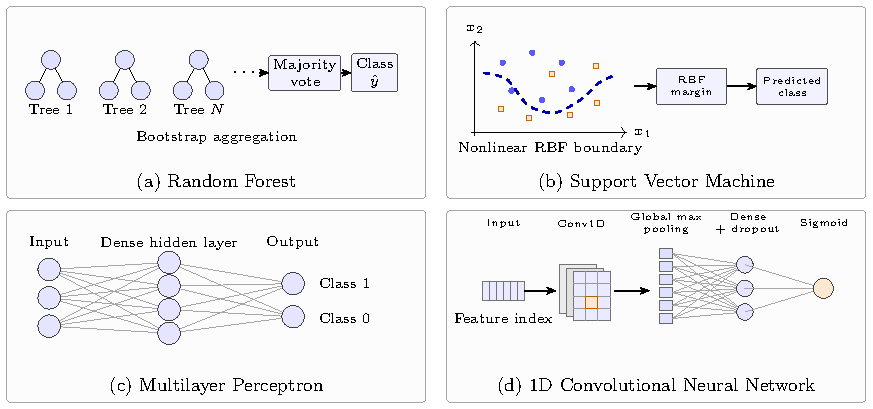
\includegraphics[width=0.9\linewidth]{figures/classifier_backbones_vector.pdf}
    \caption{Architectural topologies and structural decision mechanisms of the four candidate classifier
backbones evaluated under the equal-budget metaheuristic optimization framework.}
    \label{fig:classifier_backbones}
\end{figure}


\subsection{Optimizer Configuration, Search Operators, and Validation Objectives}
\label{sec:optimizerconfiguration}

To support a controlled comparison, five search paradigms were evaluated: Random Search (RS), Genetic Algorithm (GA), Particle Swarm Optimization (PSO), Differential Evolution (DE), and Grey Wolf Optimizer (GWO). All optimizers operate under a strict candidate evaluation cap of $N_{\mathrm{eval}} = 1{,}000$ per model and random seed. For all population-based algorithms (GA, PSO, DE, GWO), the population size is fixed to $N_{\mathrm{pop}} = 10$ candidates evaluated across $G = 100$ generations or iterations ($10 \times 100 = 1{,}000$ function evaluations). RS generates $N_{\mathrm{eval}} = 1{,}000$ independent uniform random samples across the search space.

Candidate vectors use the bounds stated above. Integer parameters and categorical-option indices are rounded and clipped to their admissible bounds:
\begin{equation}\label{eq:decoding_discrete}
\theta_d = \mathrm{clip}\!\left(\mathrm{round}(u_d),\theta_{d,\mathrm{min}},\theta_{d,\mathrm{max}}\right).
\end{equation}
For continuous parameters defined on logarithmic scales (such as $C$, $\alpha$, and learning rates), optimizers act on $u_d\in[\log_{10}(\theta_{d,\mathrm{min}}),\log_{10}(\theta_{d,\mathrm{max}})]$ and values are decoded by
\begin{equation}\label{eq:decoding_log}
\theta_d = 10^{u_d}.
\end{equation}

The specific search operators and update formulations governing each optimizer are defined as follows:
\begin{itemize}
    \item \textbf{Genetic Algorithm (GA)}: Utilizes tournament selection ($k=3$), uniform crossover with probability $P_c = 0.80$, and mutation with probability $P_m = 0.20$. When a gene is mutated, its perturbation scale is 0.10 of the corresponding encoded search range.
    \item \textbf{Particle Swarm Optimization (PSO)}: Velocity vectors $\mathbf{v}_i$ and positions $\mathbf{u}_i$ for particle $i$ at iteration $g$ are updated using inertia weight $w = 0.70$ and cognitive/social coefficients $c_1 = c_2 = 1.50$:
    \begin{equation}\label{eq:pso_update}
    \mathbf{v}_i^{g+1} = w \mathbf{v}_i^g + c_1 r_1 (\mathbf{pbest}_i - \mathbf{u}_i^g) + c_2 r_2 (\mathbf{gbest} - \mathbf{u}_i^g),
    \end{equation}
    \begin{equation}
    \mathbf{u}_i^{g+1} = \mathrm{clip}\left(\mathbf{u}_i^g + \mathbf{v}_i^{g+1}, 0, 1\right),
    \end{equation}
    where $r_1, r_2 \sim U(0, 1)$.
    \item \textbf{Differential Evolution (DE)}: Implements the DE/best/1/bin strategy with mutation factor $F = 0.80$ and binomial crossover probability $CR = 0.90$:
    \begin{equation}\label{eq:de_update}
    \mathbf{v}_i^{g+1} = \mathbf{gbest}^g + F (\mathbf{u}_{r1}^g - \mathbf{u}_{r2}^g),
    \end{equation}
    where $r1, r2$ are distinct randomly chosen population indices.
    \item \textbf{Grey Wolf Optimizer (GWO)}: Candidate position vectors are updated by simulating encirclement of the three leading wolves ($\bm{\alpha}, \bm{\beta}, \bm{\delta}$):
    \begin{equation}\label{eq:gwo_update}
    \mathbf{u}_i^{g+1} = \frac{\mathbf{x}_1 + \mathbf{x}_2 + \mathbf{x}_3}{3},
    \end{equation}
    where $\mathbf{x}_1 = \bm{\alpha} - \mathbf{A}_1 \cdot |\mathbf{C}_1 \cdot \bm{\alpha} - \mathbf{u}_i^g|$, with analogous terms for $\mathbf{x}_2$ ($\bm{\beta}$) and $\mathbf{x}_3$ ($\bm{\delta}$).
\end{itemize}

Candidate configurations are evaluated against two separated validation objectives:
\begin{itemize}
    \item \textbf{Protocol A (MCC/$F_1$ Fitness)}:
    \begin{equation}\label{eq:fitness_protocol_a}
    f_{\mathrm{MCC/F1}}(\boldsymbol{\theta}) = 0.60\,\mathrm{MCC}_{\mathrm{val}}(\boldsymbol{\theta}) + 0.40\,F_{1,\mathrm{val}}(\boldsymbol{\theta}).
    \end{equation}
    \item \textbf{Protocol B (Weighted-Accuracy Fitness)}:
    \begin{equation}\label{eq:fitness_protocol_b}
    f_{\mathrm{Acc}}(\boldsymbol{\theta}) = 0.40\,\mathrm{Accuracy}_{\mathrm{train}}(\boldsymbol{\theta}) + 0.60\,\mathrm{Accuracy}_{\mathrm{val}}(\boldsymbol{\theta}).
    \end{equation}
\end{itemize}

In addition to the two primary holdout protocols, Experiment 3 uses a separate exploratory weighted-accuracy objective with three-fold expanding-window temporal cross-validation on the concatenated training and validation observations ($N=12{,}045$). For each fold, the candidate is fitted to the earlier portion and scored on the subsequent portion; its objective is the mean of $0.40\,\mathrm{Accuracy}_{\mathrm{train}}+0.60\,\mathrm{Accuracy}_{\mathrm{validation}}$ across folds. The test feature rows are excluded from candidate selection and the selected candidate is refitted on all training-plus-validation observations before test scoring. The folds were not purged for the one-row target shift: in each fold, the last training row's target is taken from the first validation row. Experiment 3 is reported separately because its selection protocol differs from the two holdout protocols.

The two primary holdout protocols differ in both the metric and the data contribution to fitness: Protocol A uses validation MCC/$F_1$, whereas Protocol B combines in-sample training accuracy and validation accuracy. Their outcome contrast therefore describes two complete selection protocols and does not isolate the effect of changing the metric alone.

Upon completion of the $N_{\mathrm{eval}} = 1{,}000$ search budget, the optimal candidate vector $\boldsymbol{\theta}^* = \arg\max f(\boldsymbol{\theta})$ is refit on the concatenated training and validation dataset ($N = 12{,}045$ bars) and evaluated on the nominal test block ($N = 3{,}012$ feature bars). For the exploratory economic assessment, the prediction generated after bar $t$ closes is applied to bar $t+1$: an uptrend prediction opens a long position at the next bar's open, while a downtrend prediction opens a short position; each position is closed at that bar's close. The next-bar replay therefore contains at most 3,011 trades from the 3,012-row test block. Each round trip is charged a fixed cost of five index points. We report total net profit, maximum drawdown, profit factor, and annualized daily point-P\&L Sharpe ratio, computed as $\sqrt{252}\,\bar{R}_{d}/s_{d}$ from daily net point totals. These values describe this simplified one-bar execution rule, not deployable live performance. The target uses pivot-defined regime labels, whose endpoint is confirmed retrospectively; the temporal boundary implications of that labeling procedure remain a limitation of this benchmark.

\subsubsection{Asymptotic search overhead}
Let $d_s$ denote the number of encoded hyperparameters in a search space, $P$ the population size, and $G$ the number of generations or iterations. For RS, GA, PSO, and GWO, sampling and updating candidate vectors requires $O(N_{\mathrm{eval}}d_s)$ arithmetic operations when population size and tournament size are fixed; bookkeeping over fitness values adds at most $O(N_{\mathrm{eval}})$. DE also performs $O(N_{\mathrm{eval}}d_s)$ mutation, crossover, and selection work. The present DE implementation additionally constructs a list of eligible peers for each target vector, giving an implementation-specific $O(GP^2)$ bookkeeping term. Since $P=10$ is fixed in this benchmark and $N_{\mathrm{eval}}=PG$, this term is linear in the number of evaluations here. Thus, the optimizer-side overhead of all five methods is linear in $N_{\mathrm{eval}}$ for the fixed benchmark settings; this statement does not imply equal wall-clock cost.

The dominant computational cost is candidate-model fitting, not optimizer-vector arithmetic. A useful cost decomposition is $C_{\mathrm{total}}=N_{\mathrm{fit}}\,C_{\mathrm{fit}}(m,n,\boldsymbol{\theta})+C_{\mathrm{search}}$, where $m$ is the backbone, $n$ is the number of fitting observations, $\boldsymbol{\theta}$ is the candidate configuration, and $N_{\mathrm{fit}}$ counts uncached fits (three fits per uncached candidate in Experiment 3). Because RF, SVM, MLP, and 1D-CNN have different data- and parameter-dependent training costs, one common closed-form training complexity would be misleading. We therefore report an empirical fit-count measure alongside the asymptotic optimizer overhead. The candidate logs also record fit-level training seconds, used in the complementary normalized overview, but they do not provide controlled end-to-end wall-clock comparisons that include optimizer bookkeeping and orchestration.
\subsubsection{Empirical search effort}
\label{sec:empirical_effort}
The equal $N_{\mathrm{eval}}$ budget counts objective calls, but repeated candidate configurations may be served from the evaluation cache. We therefore distinguish objective calls from actual candidate-model fits. For each model--optimizer--seed run, we record the first candidate at which best-so-far validation fitness reaches 95\% of that run's total observed improvement. If $b_1$ and $b_T$ denote the initial and final best-so-far fitness, the threshold is $b_1+0.95(b_T-b_1)$. Calls to threshold equal the candidate evaluation index; actual fits equal cumulative cache misses through that index, multiplied by three for Experiment 3 (one fit per temporal fold) and one for each holdout experiment. The final refit for test evaluation is excluded. Thus, 95\% is a run-relative validation-fitness convergence threshold: it is not a 95\% test accuracy or a target defined from test performance. Held-out test metrics are computed separately after configuration selection. Values are summarized by the median across the three seeds and interpreted descriptively.

\subsection{Statistical Analysis}
\label{sec:statistical_analysis}

Statistical comparisons are conducted separately within each holdout protocol and use the four classifier backbones as the groups of interest. For a given endpoint, each optimizer--seed pair defines one matched block, giving 15 blocks (five optimizers and three seeds) per protocol. We first apply the Friedman rank test to assess whether model outcomes differ across these matched blocks. When summarizing pairwise contrasts, the model with the highest marginal mean for the endpoint is compared with each of the other three models using two-sided paired Wilcoxon signed-rank tests. The resulting three $p$-values are adjusted together using the Holm step-down procedure, with family-wise significance level $\alpha=0.05$.

These tests are exploratory. The blocks share one chronological test segment, and the five optimizers and three seeds do not provide 15 independent market periods. Accordingly, the tests quantify consistency of model ordering across the evaluated optimizer--seed combinations on this fixed test period; they do not establish replication across market regimes or a confirmatory difference between validation protocols. No optimizer-superiority claim is inferred from these model-level tests.

\section{Results}\label{sec:results}

The data partition, search budget, validation objectives, and statistical procedures are defined in Section~\ref{sec:methods}. This section focuses on the empirical patterns they produce: first the deterministic reference baselines, then optimization trajectories, test-block performance, model-level summaries, exploratory inference, and economic outcomes. Unless otherwise stated, optimizer summaries use the three common seeds; inferential blocks share the same chronological test interval and are interpreted accordingly.

\subsection{Reference Baselines}

Two deterministic reference models were evaluated on the same test block before interpreting the optimizer benchmark. The majority-direction baseline predicts the class that is more frequent in the training partition; its probability is fixed at that training prevalence. The default RF baseline uses the same fixed seven-feature representation and the final-refit rule (training plus validation), but no hyperparameter search. These references are not additional optimizers and do not enter the matched optimizer--seed statistical tests.

Table~\ref{tab:reference_baselines} establishes two fixed reference points before the tuned models are compared. The majority-direction rule attains accuracy 0.510 and $F_1=0.675$ but MCC 0, showing how the prevalent class can inflate positive-class $F_1$ without useful class association. The untuned RF improves on that rule (MCC 0.210; balanced accuracy 0.604), but remains a single-backbone reference rather than a no-tuning baseline for every architecture. Thus, optimized outcomes should be interpreted relative to these limited but informative anchors.

\begin{table}[htbp]
\centering
\caption{Test-block reference baselines under the temporal protocol. The naive baseline selects the training-majority direction (uptrend); the default RF is refitted on training plus validation with 100 trees and no hyperparameter search.}
\label{tab:reference_baselines}
\manuscripttablestyle
\begin{tabular}{lrrrrr}\toprule
\textbf{Reference} & \textbf{Accuracy} & \textbf{Bal. accuracy} & \textbf{$F_1$} & \textbf{MCC} & \textbf{AUC-ROC}\\\midrule
Naive majority direction & 0.510 & 0.500 & 0.675 & 0.000 & 0.500\\
Default RF (no tuning) & 0.605 & 0.604 & 0.630 & 0.210 & 0.645\\\bottomrule
\end{tabular}
\end{table}

The contrast in Table~\ref{tab:reference_baselines} motivates reporting MCC alongside accuracy and $F_1$: no single endpoint captures both the majority-class effect and balanced predictive association. Because only RF has a default-model reference here, the table does not support claims about the benefit of tuning for the other three backbones.

\subsection{Representative Search Configurations}
\label{sec:performance_models}

Table~\ref{tab:all_hyperparameters} summarizes the search domains and one illustrative GA-selected configuration per backbone (seed 1 under the MCC/$F_1$ protocol). The selected values span distinct regions of the stated domains, particularly for network width and learning rate, underscoring that a single example is not a model-family default. These four configurations are illustrative only; the benchmark conclusions below use all five optimizers and all three common seeds.

The RF example selects a shallow tree ensemble, while the neural-network examples select different widths, regularization, and learning-rate scales. These individual settings clarify what the search space permits but do not explain comparative performance by themselves; that evidence comes from the repeated convergence and test-block summaries.

\begin{table}[!htbp]
\centering
\caption{Hyperparameter search domains and representative GA-selected configurations (seed 1 under MCC/$F_1$ fitness) across the four classifier backbones.}
\label{tab:all_hyperparameters}
\manuscripttablestyle
\begin{tabularx}{0.95\linewidth}{@{}>{\raggedright\arraybackslash}p{0.30\linewidth}X>{\centering\arraybackslash}p{0.16\linewidth}@{}}
\toprule
\multicolumn{3}{@{}l}{\textbf{Panel A: Random Forest (RF)}}\\
\textbf{Hyperparameter} & \textbf{Search space} & \textbf{Selected}\\\midrule
$n_{\mathrm{estimators}}$ & $[50,500]$ & 58\\
$\mathrm{max\_depth}$ & $[5,50]$ & 6\\
$\mathrm{min\_samples\_split}$ & $[2,20]$ & 13\\
$\mathrm{min\_samples\_leaf}$ & $[1,20]$ & 15\\
$\mathrm{max\_features}$ & $\{\mathrm{sqrt},\mathrm{log2},\mathrm{None}\}$ & None\\
$\mathrm{class\_weight}$ & $\{\mathrm{None},\mathrm{balanced}\}$ & None\\
\addlinespace[3pt]
\multicolumn{3}{@{}l}{\textbf{Panel B: Support Vector Machine (SVM)}}\\
\textbf{Hyperparameter} & \textbf{Search space} & \textbf{Selected}\\\midrule
$C$ & $[10^{-3},10^{3}]$ (log scale) & 2.089\\
$\gamma$ & $[10^{-5},10^{1}]$ (log scale) & 5.044\\
Kernel & $\{\mathrm{linear},\mathrm{RBF}\}$ & linear\\
\addlinespace[3pt]
\multicolumn{3}{@{}l}{\textbf{Panel C: Multilayer Perceptron (MLP)}}\\
\textbf{Hyperparameter} & \textbf{Search space} & \textbf{Selected}\\\midrule
Hidden neurons & $[5,500]$ & 410\\
Learning rate & $[10^{-8},10^{-2}]$ (log scale) & $3.42\times10^{-4}$\\
$L_2$ regularization & $[10^{-8},10^{-2}]$ (log scale) & $1.66\times10^{-7}$\\
Dropout rate & $[0,0.10]$ & 0.057\\
Batch size & $\{16,32,64,80,112,128\}$ & 112\\
\addlinespace[3pt]
\multicolumn{3}{@{}l}{\textbf{Panel D: 1D Convolutional Neural Network (1D-CNN)}}\\
\textbf{Hyperparameter} & \textbf{Search space} & \textbf{Selected}\\\midrule
Filters & $[8,128]$ & 48\\
Kernel size & $[2,5]$ & 3\\
Dense neurons & $[16,256]$ & 251\\
Learning rate & $[10^{-8},10^{-2}]$ (log scale) & $3.90\times10^{-6}$\\
$L_2$ regularization & $[10^{-8},10^{-2}]$ (log scale) & $5.70\times10^{-6}$\\
Dropout rate & $[0,0.10]$ & 0.026\\
Batch size & $\{16,32,64,80,112,128\}$ & 16\\
\bottomrule
\end{tabularx}
\end{table}
\FloatBarrier

\subsubsection{Random Forest}

Figures~\ref{fig:rf_convergence_mccf1} and~\ref{fig:rf_convergence_accuracy} show rapid early improvement under both fitness protocols. Under MCC/$F_1$ fitness, the five trajectories approach a near-plateau early; thereafter RS continues a modest stepwise rise, while GA remains below the close DE, PSO, and GWO terminal values. Under weighted-accuracy fitness, the curves again rise sharply at the beginning and then change little, with narrow terminal separation and GWO slightly higher. Most progress therefore occurs well before the 1,000-evaluation limit. The endpoint gaps, particularly among the population methods, are descriptive and do not establish optimizer superiority.

The RF panels differ mainly in the extent of late refinement: the MCC/$F_1$ trajectories retain somewhat more separation, whereas weighted-accuracy fitness ends in a tightly grouped set. Neither panel suggests a large payoff from spending the entire budget after the initial gains.


\subsubsection{Support Vector Machine}

Figures~\ref{fig:svm_convergence_mccf1} and~\ref{fig:svm_convergence_accuracy} display the strongest optimizer sensitivity. Under MCC/$F_1$ fitness, GWO and PSO make larger later gains and finish above RS and DE, while GA levels off at a lower fitness. Under weighted-accuracy fitness, GWO, PSO, and RS form a close upper group, DE finishes lower, and GA is lowest. These distinctions remain visible in the terminal insets, despite a common evaluation budget.

This search sensitivity is consistent with the wide SVM test-block dispersion in Table~\ref{tab:predictive_summary}. However, validation ranking does not determine the test ranking: under MCC/$F_1$ fitness, GA has the largest mean test MCC (0.290), although its validation-fitness trajectory finishes below GWO and PSO. Under weighted-accuracy fitness, GWO leads both the validation trajectory and the test-accuracy means, an alignment observed here rather than a general guarantee.


\subsubsection{Multilayer Perceptron}

Figures~\ref{fig:mlp_convergence_mccf1} and~\ref{fig:mlp_convergence_accuracy} reveal objective-dependent behaviour. With MCC/$F_1$ fitness, DE, PSO, GA, and GWO largely flatten during the later budget, whereas RS continues to improve and finishes above the other curves. That visual validation advantage does not carry through to test-block MCC: RS averages 0.106, compared with 0.305 for GWO and 0.302 for DE in Table~\ref{tab:optimizer_primary_metrics}. Under weighted-accuracy fitness, all five trajectories become tightly clustered after their early gains and remain nearly indistinguishable near termination.

The MLP curves show why visually similar terminal validation fitness must not be treated as identical generalization: under weighted-accuracy fitness, the test-block means still span optimizer-specific values, while the MCC/$F_1$ panel's late RS advantage is paired with the lowest RS test MCC. These descriptive contrasts indicate that the objective shapes the selected search region, but do not establish why a particular configuration generalizes better.


\subsubsection{One-Dimensional Convolutional Neural Network}

Figures~\ref{fig:cnn_convergence_mccf1} and~\ref{fig:cnn_convergence_accuracy} show rapid early progress followed by a stable tail. Under MCC/$F_1$ fitness, PSO and GWO end at the upper edge of a compact group; GA and DE level off slightly lower, and RS lies between them. Under weighted-accuracy fitness, trajectories are again close after the initial rise, with GWO finishing marginally above the others. Relative to SVM, optimizer separation is narrower, especially for the weighted-accuracy trajectory.

The test table qualifies these small validation gaps. Under MCC/$F_1$ fitness, PSO has the largest mean test MCC (0.269), while GWO's test MCC is 0.139 despite its near-leading validation trajectory. Under weighted-accuracy fitness, GWO also has the largest mean test accuracy (0.637), but the other four means are close (0.634--0.636). 

\begin{figure}[H]
\centering
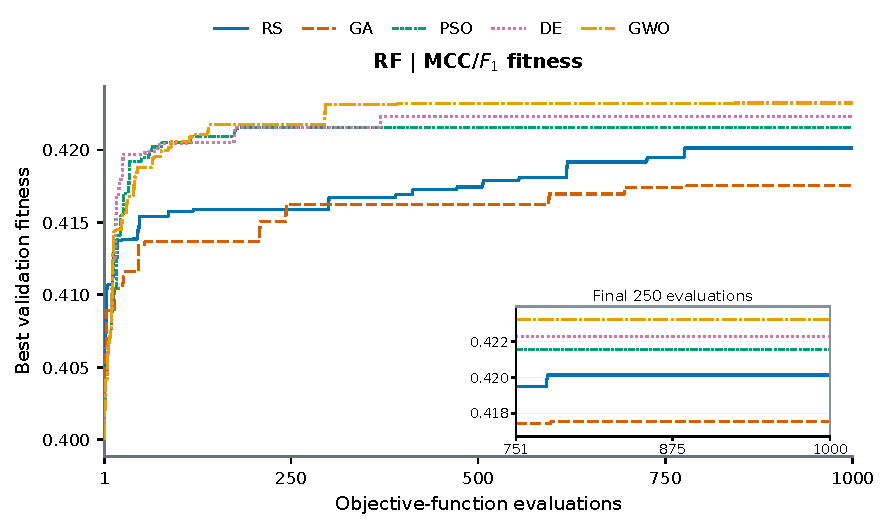
\includegraphics[width=0.90\linewidth]{figures/rf_convergence_mccf1.pdf}
\caption{Best-so-far validation fitness over 1,000 objective-function evaluations for RF under MCC/$F_1$ fitness. Curves show mean fitness across the three common seeds for RS, GA, PSO, DE, and GWO; the inset covers evaluations 751--1,000.}
\label{fig:rf_convergence_mccf1}
\end{figure}

\begin{figure}[H]
\centering
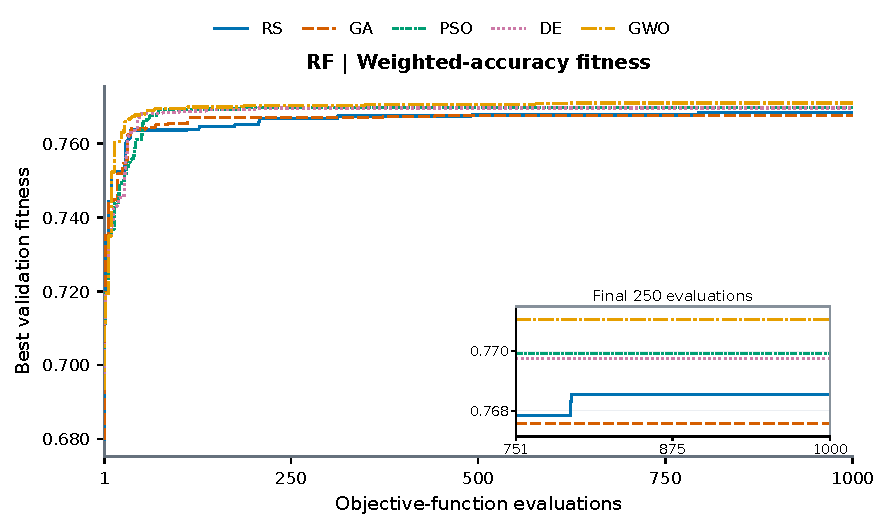
\includegraphics[width=0.90\linewidth]{figures/rf_convergence_accuracy.pdf}
\caption{Best-so-far validation fitness over 1,000 objective-function evaluations for RF under weighted-accuracy fitness. Curves show mean fitness across the three common seeds for RS, GA, PSO, DE, and GWO; the inset covers evaluations 751--1,000.}
\label{fig:rf_convergence_accuracy}
\end{figure}

\begin{figure}[!p]
\centering
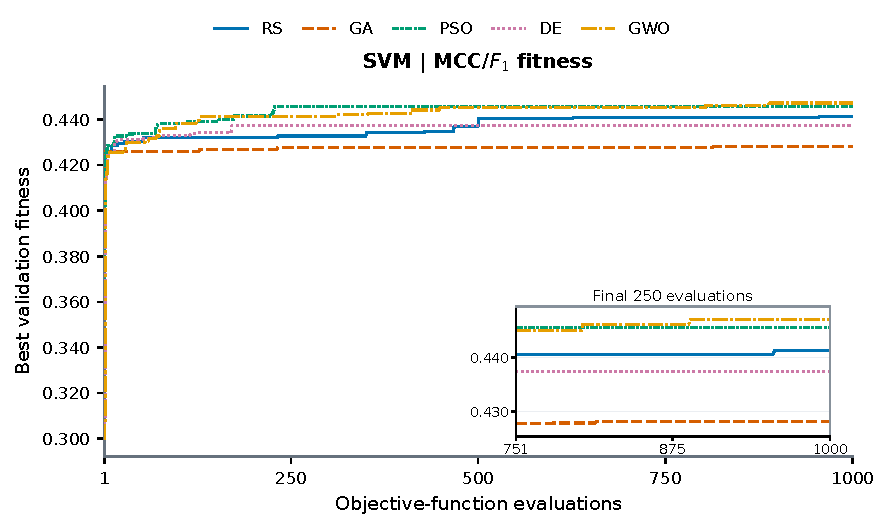
\includegraphics[width=0.90\linewidth]{figures/svm_convergence_mccf1.pdf}
\caption{Best-so-far validation fitness over 1,000 objective-function evaluations for SVM under MCC/$F_1$ fitness. Curves show mean fitness across the three common seeds for RS, GA, PSO, DE, and GWO; the inset covers evaluations 751--1,000.}
\label{fig:svm_convergence_mccf1}
\end{figure}

\begin{figure}[!p]
\centering
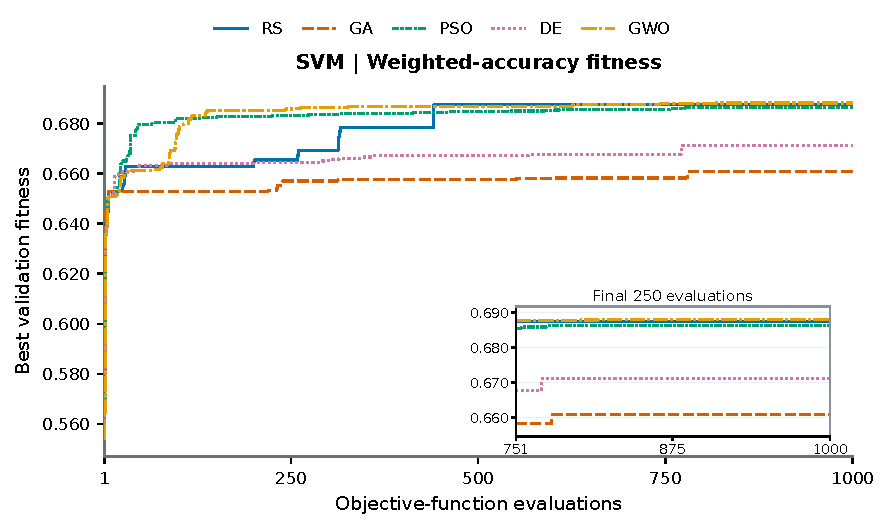
\includegraphics[width=0.90\linewidth]{figures/svm_convergence_accuracy.pdf}
\caption{Best-so-far validation fitness over 1,000 objective-function evaluations for SVM under weighted-accuracy fitness. Curves show mean fitness across the three common seeds for RS, GA, PSO, DE, and GWO; the inset covers evaluations 751--1,000.}
\label{fig:svm_convergence_accuracy}
\end{figure}

\begin{figure}[!p]
\centering
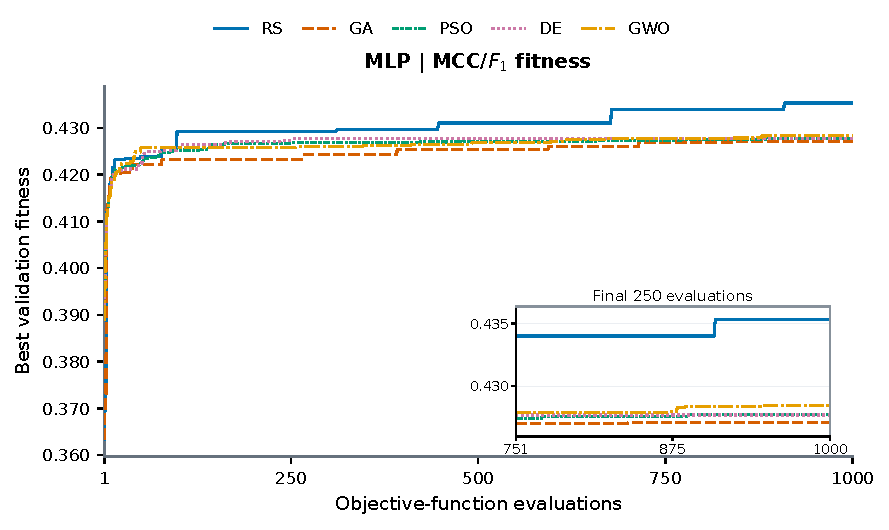
\includegraphics[width=0.90\linewidth]{figures/mlp_convergence_mccf1.pdf}
\caption{Best-so-far validation fitness over 1,000 objective-function evaluations for MLP under MCC/$F_1$ fitness. Curves show mean fitness across the three common seeds for RS, GA, PSO, DE, and GWO; the inset covers evaluations 751--1,000.}
\label{fig:mlp_convergence_mccf1}
\end{figure}

\begin{figure}[!p]
\centering
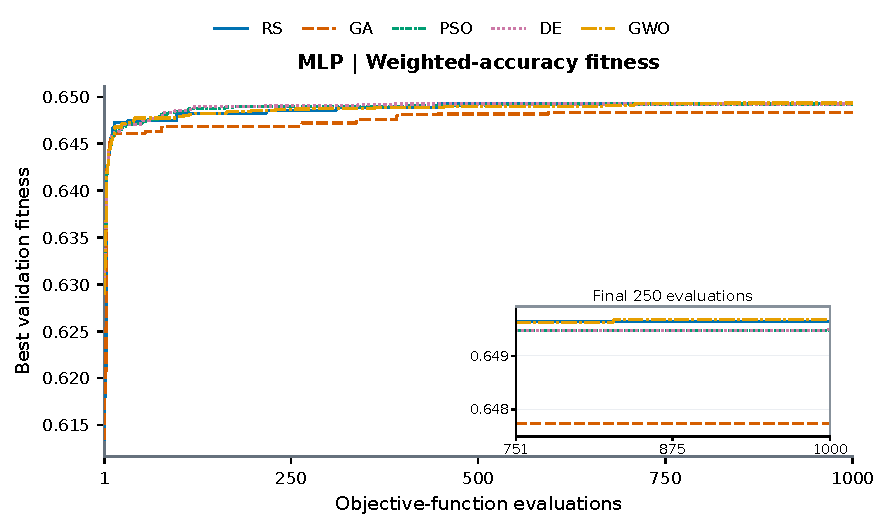
\includegraphics[width=0.90\linewidth]{figures/mlp_convergence_accuracy.pdf}
\caption{Best-so-far validation fitness over 1,000 objective-function evaluations for MLP under weighted-accuracy fitness. Curves show mean fitness across the three common seeds for RS, GA, PSO, DE, and GWO; the inset covers evaluations 751--1,000.}
\label{fig:mlp_convergence_accuracy}
\end{figure}

\begin{figure}[!p]
\centering
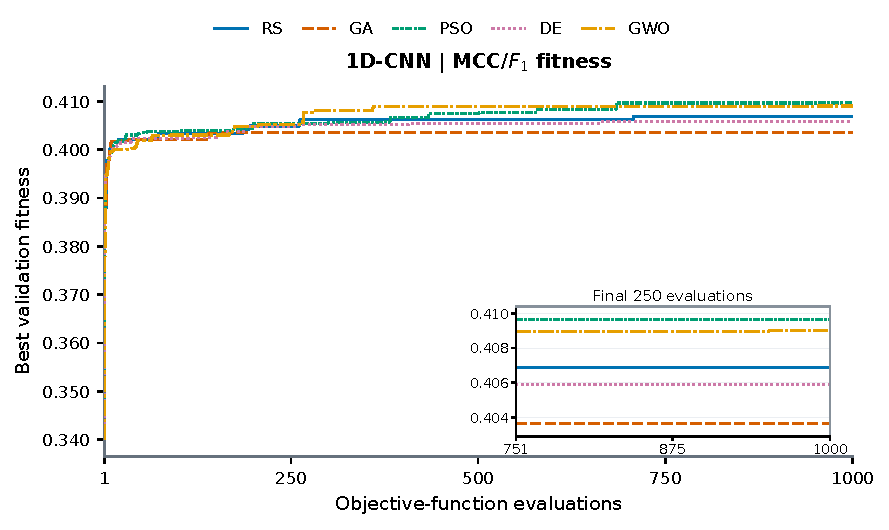
\includegraphics[width=0.90\linewidth]{figures/cnn_convergence_mccf1.pdf}
\caption{Best-so-far validation fitness over 1,000 objective-function evaluations for 1D-CNN under MCC/$F_1$ fitness. Curves show mean fitness across the three common seeds for RS, GA, PSO, DE, and GWO; the inset covers evaluations 751--1,000.}
\label{fig:cnn_convergence_mccf1}
\end{figure}

\begin{figure}[!p]
\centering
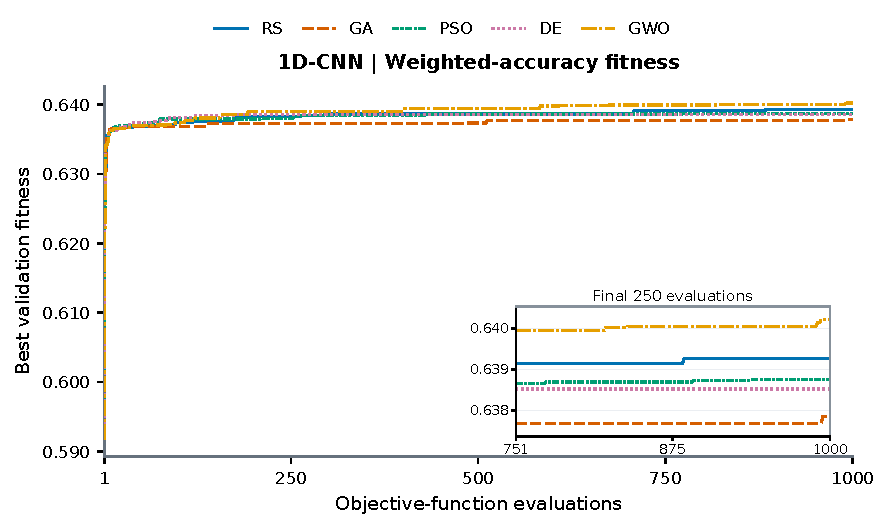
\includegraphics[width=0.90\linewidth]{figures/cnn_convergence_accuracy.pdf}
\caption{Best-so-far validation fitness over 1,000 objective-function evaluations for 1D-CNN under weighted-accuracy fitness. Curves show mean fitness across the three common seeds for RS, GA, PSO, DE, and GWO; the inset covers evaluations 751--1,000.}
\label{fig:cnn_convergence_accuracy}
\end{figure}

\FloatBarrier

\subsection{Optimizer-Level Performance Under Equal Budget}

Convergence describes selection on validation fitness, not performance on the held-out period. Table~\ref{tab:optimizer_primary_metrics} therefore compares the test-block endpoint aligned with each validation protocol: MCC for MCC/$F_1$ fitness and accuracy for weighted-accuracy fitness. Entries are means over three common seeds under the same 1,000-evaluation budget; they are descriptive summaries, not tests of optimizer superiority.

\begin{table}[htbp]
\centering
\caption{Optimizer-level test-block primary metrics under equal budget. Each cell is a mean over three common seeds; boldface denotes the largest mean within a model and protocol.}
\label{tab:optimizer_primary_metrics}
\manuscripttablestyle
\begin{tabular}{lccccc}\toprule
\textbf{Model} & \textbf{RS} & \textbf{GA} & \textbf{PSO} & \textbf{DE} & \textbf{GWO}\\\midrule
\multicolumn{6}{c}{\textbf{Panel A: MCC/$F_1$ fitness; test-block MCC}}\\\midrule
RF & 0.281 & \textbf{0.293} & 0.293 & 0.292 & 0.288\\
SVM & 0.105 & \textbf{0.290} & 0.255 & 0.187 & 0.232\\
MLP & 0.106 & 0.290 & 0.299 & 0.302 & \textbf{0.305}\\
1D-CNN & 0.179 & 0.268 & \textbf{0.269} & 0.267 & 0.139\\\midrule
\multicolumn{6}{c}{\textbf{Panel B: weighted-accuracy fitness; test-block accuracy}}\\\midrule
RF & 0.604 & \textbf{0.611} & 0.604 & 0.600 & 0.602\\
SVM & 0.588 & 0.557 & 0.571 & 0.584 & \textbf{0.593}\\
MLP & 0.649 & 0.649 & \textbf{0.652} & 0.652 & 0.652\\
1D-CNN & 0.636 & 0.634 & 0.635 & 0.634 & \textbf{0.637}\\\bottomrule
\end{tabular}
\end{table}

The table shows an optimizer-by-model interaction rather than a common winner. Under MCC/$F_1$ fitness, RF is comparatively insensitive among GA, PSO, and DE (0.293, 0.293, and 0.292), whereas its RS mean is 0.281. SVM is more sensitive: GA reaches 0.290, but RS reaches only 0.105; for MLP, GWO is highest at 0.305 while RS is again 0.106. The 1D-CNN is tightly grouped across GA, PSO, and DE (0.267--0.269), but lower for RS and particularly GWO. Under weighted-accuracy fitness, the five MLP means are tightly clustered (0.649--0.652); the SVM range is wider (0.557--0.593), while RF spans 0.600--0.611 and 1D-CNN spans 0.634--0.637. Thus, optimizer sensitivity depends on both the backbone and the selected endpoint. With only three common seeds, the within-row maxima are not evidence of a universally best optimizer; the cross-backbone summary in Table~\ref{tab:predictive_summary} describes how the model ordering changes between the primary protocols.

\subsection{Model-Level Aggregation Across Optimizers}
Table~\ref{tab:predictive_summary} summarizes the two primary holdout protocols over 15 optimizer--seed blocks per backbone. Experiment 3 uses a distinct temporal cross-validation selection procedure and is therefore shown separately below. These holdout summaries are descriptive and do not represent 15 independent market replications.

\begin{table}[!htbp]
\centering
\caption{Test-block predictive outcomes by backbone and validation protocol. Entries are mean $\pm$ standard deviation over 15 optimizer--seed blocks per row (five optimizers $\times$ three common seeds).}
\label{tab:predictive_summary}
\manuscripttablestyle
\begin{tabular}{lrrr}\toprule
\multicolumn{4}{c}{\textbf{Panel A: MCC/$F_1$ validation fitness}}\\\midrule
\textbf{Model} & Accuracy & MCC & $F_1$\\\midrule
RF & $0.645\pm0.004$ & $0.289\pm0.008$ & $0.664\pm0.006$\\
SVM & $0.604\pm0.060$ & $0.214\pm0.132$ & $0.602\pm0.122$\\
MLP & $0.630\pm0.070$ & $0.261\pm0.141$ & $0.639\pm0.071$\\
1D-CNN & $0.613\pm0.056$ & $0.224\pm0.120$ & $0.597\pm0.166$\\\midrule
\multicolumn{4}{c}{\textbf{Panel B: Weighted-accuracy validation fitness}}\\\midrule
\textbf{Model} & Accuracy & MCC & $F_1$\\\midrule
RF & $0.604\pm0.005$ & $0.208\pm0.009$ & $0.624\pm0.004$\\
SVM & $0.578\pm0.028$ & $0.159\pm0.053$ & $0.600\pm0.071$\\
MLP & $0.651\pm0.003$ & $0.301\pm0.005$ & $0.658\pm0.004$\\
1D-CNN & $0.635\pm0.002$ & $0.271\pm0.005$ & $0.639\pm0.007$\\\bottomrule
\end{tabular}
\end{table}

In Panel A of Table~\ref{tab:predictive_summary}, RF has the highest aggregate mean for accuracy, MCC, and $F_1$, and its standard deviations are small (0.004, 0.008, and 0.006). SVM, MLP, and 1D-CNN show appreciably larger dispersion, especially for MCC/$F_1$ selection. Panel B reverses the leading backbone: MLP has the highest mean across all three metrics and low dispersion; 1D-CNN is also competitive, while RF's mean accuracy and MCC are lower than in Panel A. The pattern suggests that the validation objective changes which model/configuration regions the search favours; it does not establish that either objective is globally superior.



Figure~\ref{fig:exp1_mcc} isolates MCC for the MCC/$F_1$ holdout experiment, while Figure~\ref{fig:holdout_accuracy} compares accuracy across the two holdout experiments using the same endpoint. This separation avoids visually treating MCC and accuracy as interchangeable scales. The figures show means and seed-level standard deviations; Table~\ref{tab:predictive_summary} retains the exact backbone-level holdout summaries.

\begin{figure}[!htbp]\centering
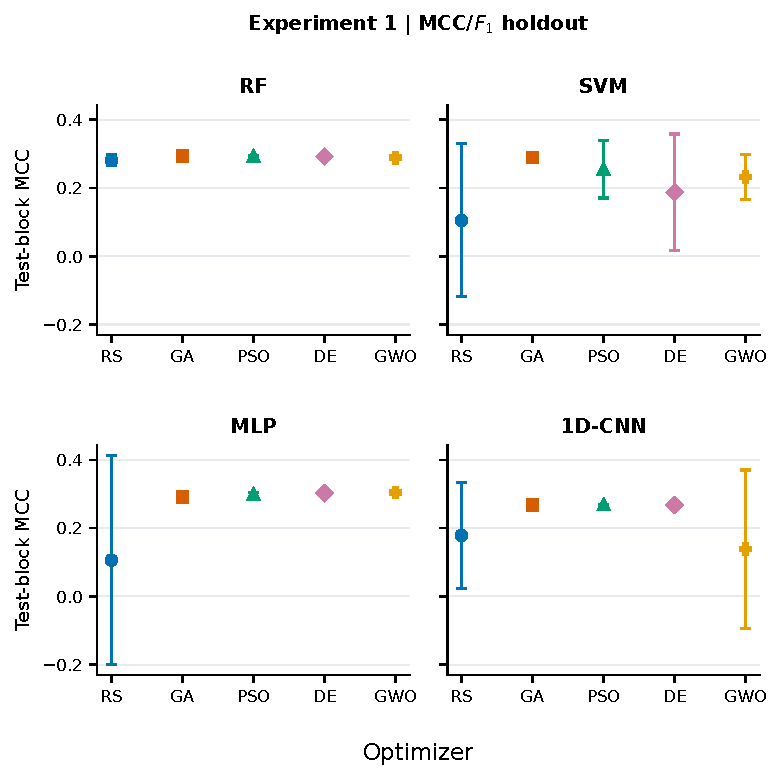
\includegraphics[width=0.95\linewidth]{figures/exp1_holdout_mcc_by_optimizer.pdf}
\caption{Test-block MCC for Experiment 1, which selects configurations using MCC/$F_1$ fitness under temporal holdout. Points show means and error bars show standard deviations across three common seeds for each optimizer and backbone.}
\label{fig:exp1_mcc}\end{figure}

\begin{figure}[!htbp]\centering
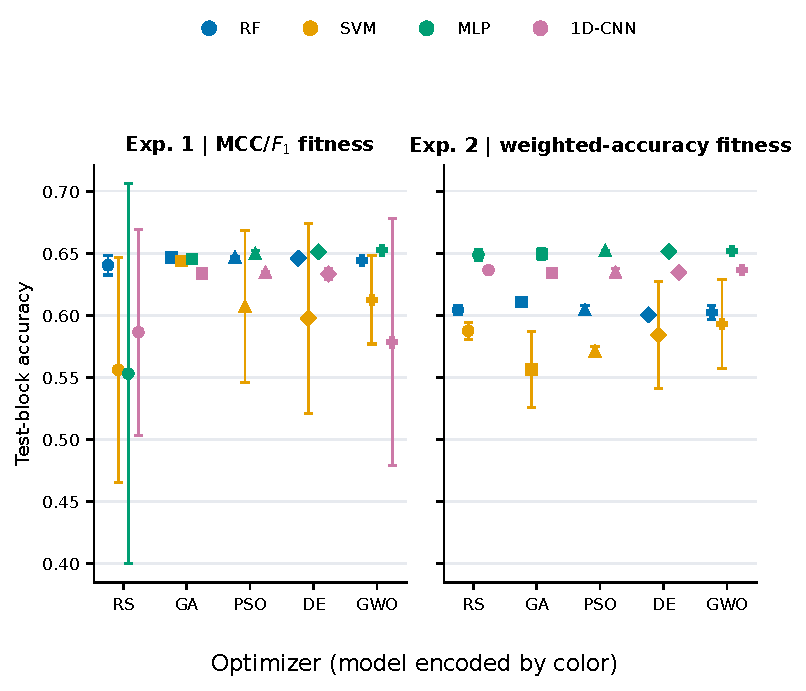
\includegraphics[width=0.95\linewidth]{figures/exp1_exp2_holdout_accuracy.pdf}
\caption{Test-block accuracy under the two temporal holdout experiments. Experiment 1 selects with MCC/$F_1$ fitness and Experiment 2 with weighted-accuracy fitness. Points show means and error bars show standard deviations across three common seeds; color identifies the backbone.}
\label{fig:holdout_accuracy}\end{figure}

On the common holdout endpoint, MLP has the largest observed mean accuracy in both experiments (0.653 for Experiment 1 with GWO; 0.652 for Experiment 2 with PSO). This agreement in accuracy does not imply that the selection objectives are equivalent: Table~\ref{tab:predictive_summary} shows different dispersion and the separately reported MCC pattern. With three seeds and one chronological test interval, these mean differences remain descriptive.

\subsection{Exploratory Temporal Cross-Validation (Experiment 3)}
\label{sec:exp3_cv}
Experiment 3 applies the weighted-accuracy objective to three expanding temporal folds formed from the training-plus-validation observations; it is kept separate from the two holdout experiments. Figure~\ref{fig:exp3_cv_accuracy} reports its test-block accuracy by optimizer and backbone. MLP again has the highest observed optimizer--backbone mean (0.652 for GWO), with its five optimizer means tightly grouped; the SVM outcomes vary more across optimizers. The test interval remains the same chronological block used in the holdout experiments, so this is an alternative selection-protocol analysis rather than an independent market replication or an additional holdout block.

\begin{figure}[!htbp]\centering
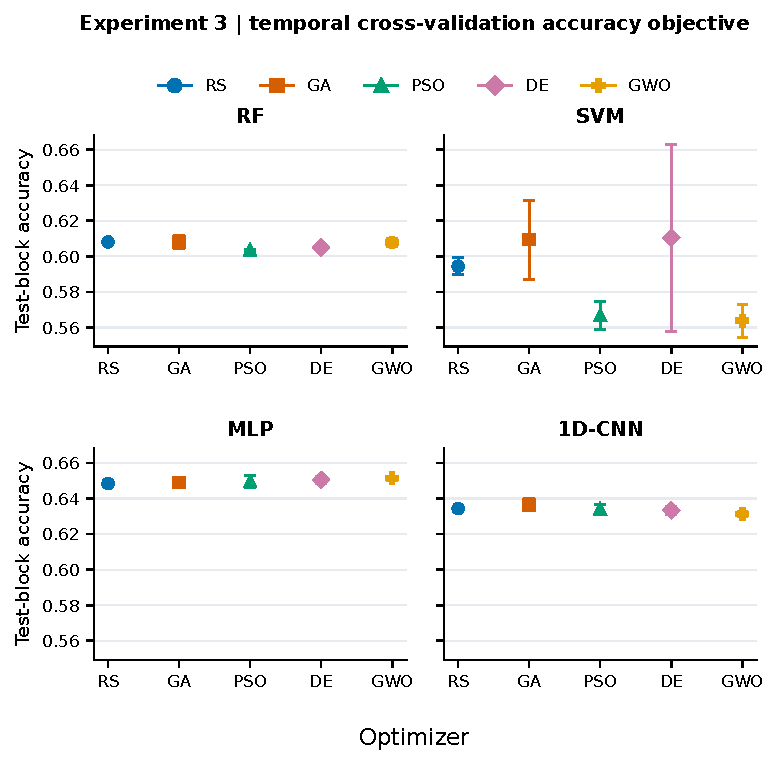
\includegraphics[width=0.95\linewidth]{figures/exp3_temporal_cv_accuracy_by_optimizer.pdf}
\caption{Test-block accuracy after configuration selection with the weighted-accuracy objective under three-fold temporal cross-validation (Experiment 3). Points show means and error bars show standard deviations across three common seeds for each optimizer and backbone.}
\label{fig:exp3_cv_accuracy}\end{figure}

\FloatBarrier
\subsection{Objective Calls and Training Effort}
\label{sec:training_effort}
Figure~\ref{fig:practical_fit_cost} compares practical search effort across the three experiments. The plotted 95\% point is a run-relative threshold on validation-fitness gain, not 95\% test accuracy or test performance. It required many fits for RS in some MCC/$F_1$ cells (619 for RF and 678 for MLP), but few in others (29 for RF under weighted-accuracy holdout); several directed methods also required hundreds of fits in selected cells. Thus, RS can lag in particular model--objective combinations, but its relative effort depends on the backbone and protocol. These results do not establish a universal optimizer ranking or a common quality-versus-cost frontier.

\begin{figure}[H]\centering
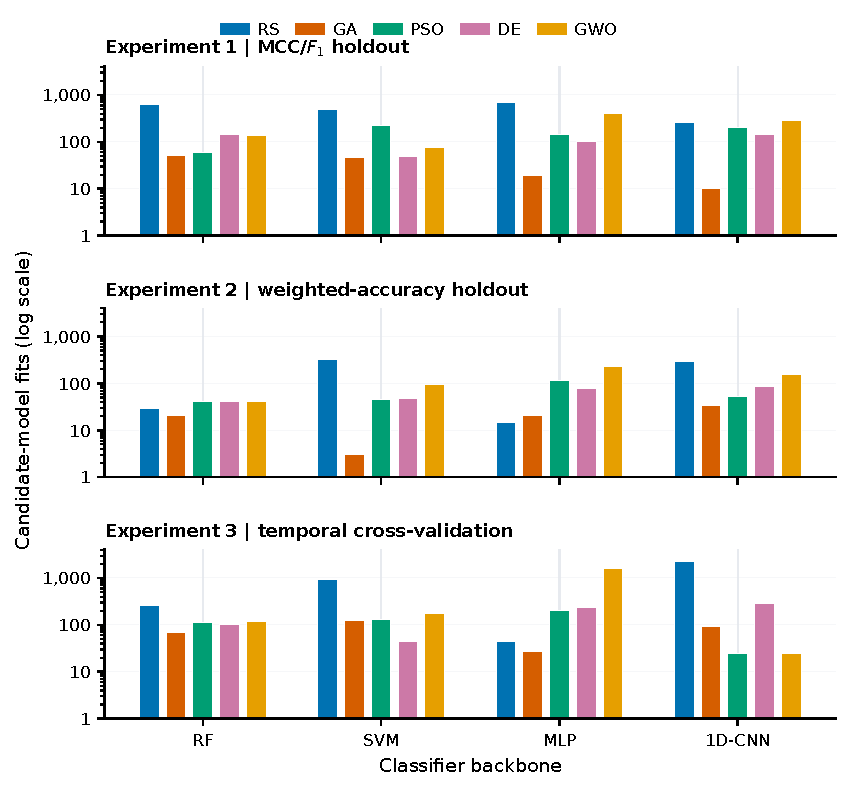
\includegraphics[width=0.95\linewidth]{figures/practical_candidate_fit_cost.pdf}
\caption{Practical search effort measured as the median number of uncached candidate-model fits needed to reach 95\% of each run's own validation-fitness gain. This threshold is computed from validation fitness and is not a test-performance target. Bars are grouped by backbone and optimizer; panels show the two holdout protocols and exploratory temporal cross-validation. The vertical axis is logarithmic. Experiment 3 counts one model fit per fold (three per uncached candidate). Lower bars indicate fewer fits to that run's own relative threshold, not fewer fits to attain a common absolute fitness.}
\label{fig:practical_fit_cost}\end{figure}

Table~\ref{tab:training_effort} gives the corresponding medians of objective calls and actual candidate-model fits to threshold, with paired calls/fits aggregated across the three seeds in each model--optimizer cell. Across cells, median actual fits to threshold were 143 for Experiment 1, 46 for Experiment 2, and 149 for Experiment 3; run-level ranges were broad (2--956, 2--708, and 6--3{,}000, respectively). Under the full 1,000-call budget, median total candidate-fit counts were 902, 970, and 2{,}702 per run, respectively. Experiment 3 has three fits for each uncached candidate because it evaluates three folds.

\begin{table}[!htbp]
\centering
\caption{Median objective calls / actual candidate-model fits to reach 95\% of the run-specific validation-fitness gain. Values are medians across three seeds; Experiment 3 counts one fit per temporal fold.}
\label{tab:training_effort}
\manuscripttablestyle
\begin{tabular}{llrrrrr}\toprule
\textbf{Experiment} & \textbf{Model} & \textbf{RS} & \textbf{GA} & \textbf{PSO} & \textbf{DE} & \textbf{GWO}\\\midrule
\multicolumn{7}{c}{\textbf{Panel A: Experiment 1, MCC/$F_1$ holdout}}\\\midrule
 & RF & 619/619 & 595/51 & 61/60 & 175/145 & 140/140\\
 & SVM & 501/501 & 780/46 & 225/224 & 53/49 & 75/75\\
 & MLP & 678/678 & 39/19 & 142/141 & 102/100 & 412/412\\
 & 1D-CNN & 262/262 & 10/10 & 200/199 & 151/145 & 280/280\\\midrule
\multicolumn{7}{c}{\textbf{Panel B: Experiment 2, weighted-accuracy holdout}}\\\midrule
 & RF & 29/29 & 32/21 & 43/41 & 42/42 & 42/42\\
 & SVM & 316/316 & 3/3 & 46/45 & 47/47 & 96/96\\
 & MLP & 15/15 & 56/21 & 114/113 & 79/78 & 229/229\\
 & 1D-CNN & 295/295 & 140/33 & 54/53 & 85/85 & 156/156\\\midrule
\multicolumn{7}{c}{\textbf{Panel C: Experiment 3, temporal cross-validation}}\\\midrule
 & RF & 86/258 & 37/69 & 40/114 & 34/102 & 40/120\\
 & SVM & 316/948 & 780/126 & 44/129 & 15/45 & 58/171\\
 & MLP & 15/45 & 9/27 & 70/207 & 82/234 & 534/1,602\\
 & 1D-CNN & 764/2,292 & 242/93 & 8/24 & 98/285 & 8/24\\\bottomrule
\end{tabular}
\end{table}

Calls and fits can differ substantially when the cache reuses a candidate, particularly for GA. Accordingly, equal objective-call budgets do not always imply equal numbers of new model fits, and the tripled cross-validation fit count should not be read as three independent test evaluations. Since the stopping point is computed separately from each run's terminal improvement, lower counts alone do not demonstrate superior predictive quality; they should be read alongside the test-block metrics above.


\subsection{Exploratory Statistical Evidence}

We compared the four backbones using Friedman tests on protocol-aligned test-block endpoints: MCC for MCC/$F_1$ fitness and accuracy for weighted-accuracy fitness. Each test contains $n=15$ matched optimizer--seed blocks (five optimizers crossed with three common seeds). For MCC/$F_1$, $\chi^2=22.840$ ($p=4.36\times10^{-5}$), with mean ranks RF 2.067, SVM 2.733, MLP 1.533, and 1D-CNN 3.667. For weighted-accuracy fitness, $\chi^2=42.920$ ($p=2.56\times10^{-9}$), with mean ranks RF 3.133, SVM 3.867, MLP 1.000, and 1D-CNN 2.000. Lower mean rank indicates a more favourable within-block ordering.

Under MCC/$F_1$, RF has the largest marginal mean MCC in Table~\ref{tab:predictive_summary}, whereas MLP has the lowest block-wise mean rank; this is not contradictory. Marginal means aggregate metric magnitudes across blocks, while mean ranks first order backbones within each block and then average those ranks. Under weighted-accuracy fitness, MLP leads both mean accuracy and mean rank; its Holm-adjusted contrasts against RF, SVM, and 1D-CNN are significant ($p_{\mathrm{Holm}}\approx0.00194$) within this analysis. These results are exploratory: the 15 blocks share one chronological market test interval and are not independent market replications, so they do not establish replication across regimes or confirmatory superiority.

\subsection{Exploratory Economic Evaluation}
Figure~\ref{fig:economic_comparison} and
Table~\ref{tab:economic_summary} compare return and downside risk when each prediction is executed on the following five-minute bar. The table reports net profit and maximum drawdown with dispersion, alongside mean profit factor and annualized daily Sharpe; the figure places mean return against mean drawdown. This joint view is important because total profit alone does not represent a complete return--risk profile.

\begin{figure}[!htbp]\centering
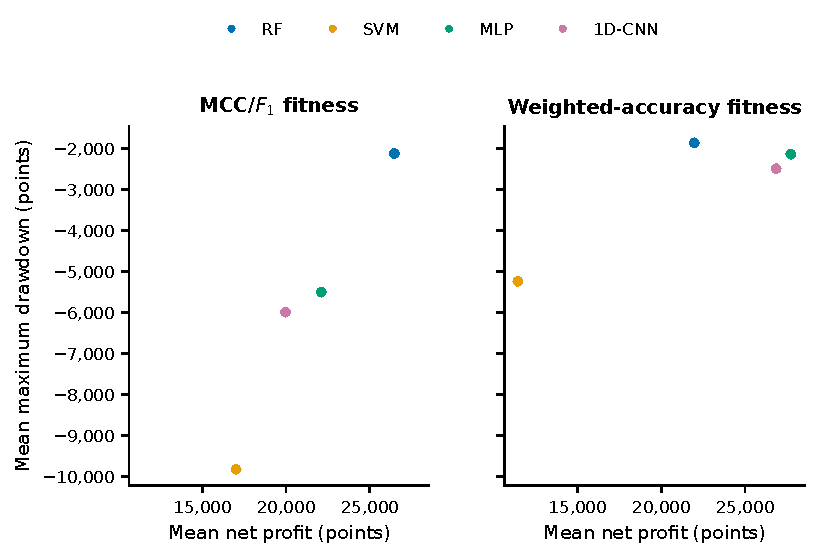
\includegraphics[width=0.95\linewidth]{figures/economic_return_drawdown.pdf}
\caption{Mean next-bar net profit versus mean maximum drawdown by backbone under MCC/$F_1$ and weighted-accuracy fitness. Each signal enters at the next five-minute bar open and exits at its close; values aggregate 15 optimizer--seed blocks. Both axes are in points, and a drawdown closer to zero indicates a smaller peak-to-trough loss.}
\label{fig:economic_comparison}\end{figure}

\begin{table}[!htbp]
\centering
\caption{Exploratory economic outcomes under the one-bar-ahead execution rule, aggregated over 15 optimizer--seed blocks per model and protocol. Signals enter at the next five-minute bar open and exit at its close. Net profit and maximum drawdown (Max. DD; points) are mean $\pm$ standard deviation; profit factor (PF) and annualized daily Sharpe ratio are means.}
\label{tab:economic_summary}
\manuscripttablestyle
\begin{tabular}{lrrrr}\toprule
\multicolumn{5}{c}{\textbf{Panel A: MCC/$F_1$ fitness}}\\\midrule
\textbf{Model} & \textbf{Net profit (points)} & \textbf{Max. DD (points)} & \textbf{PF} & \textbf{Sharpe}\\\midrule
RF & $521\pm1{,}494$ & $-4{,}567\pm251$ & 1.008 & 0.279\\
SVM & $-4{,}268\pm18{,}340$ & $-11{,}748\pm14{,}575$ & 0.967 & -0.637\\
MLP & $91\pm10{,}520$ & $-7{,}111\pm8{,}690$ & 1.010 & 0.460\\
1D-CNN & $3{,}330\pm13{,}219$ & $-7{,}871\pm9{,}866$ & 1.065 & 1.781\\\midrule
\multicolumn{5}{c}{\textbf{Panel B: weighted-accuracy fitness}}\\\midrule
\textbf{Model} & \textbf{Net profit (points)} & \textbf{Max. DD (points)} & \textbf{PF} & \textbf{Sharpe}\\\midrule
RF & $-2{,}665\pm856$ & $-4{,}979\pm548$ & 0.962 & -1.938\\
SVM & $-11{,}551\pm7{,}470$ & $-14{,}182\pm5{,}612$ & 0.851 & -5.485\\
MLP & $2{,}505\pm1{,}068$ & $-5{,}030\pm88$ & 1.037 & 1.351\\
1D-CNN & $6{,}933\pm2{,}264$ & $-4{,}917\pm93$ & 1.106 & 2.907\\\bottomrule
\end{tabular}
\end{table}

The next-bar return--risk comparison in Figure~\ref{fig:economic_comparison} shows a clear difference across backbones and protocols. Under MCC/$F_1$ fitness, 1D-CNN has the largest mean net profit (3,330 points), whereas RF has the least negative mean drawdown (-4,567 points) and the smallest drawdown dispersion. Under weighted-accuracy fitness, 1D-CNN leads mean net profit (6,933 points), profit factor (1.106), and annualized daily Sharpe (2.907); it also has a slightly less negative mean drawdown than RF. Large between-block dispersion remains for several cells, so these are exploratory outcomes under one fixed test interval and a simplified execution rule, not a trading recommendation or a transaction-cost-complete assessment.

\subsection{Complementary Benchmark Diagnostics}
\label{sec:benchmark_diagnostics}

The tables above provide compact summaries, but averaging can conceal interactions between a backbone and an optimizer. Figures~\ref{fig:heatmap_mccf1_mcc_test} and~\ref{fig:heatmap_accuracy_accuracy_test} therefore show the protocol-aligned test-block endpoint for every backbone--optimizer cell. Each cell reports the mean and standard deviation across the three common seeds; color encodes the mean.

The heatmaps make the optimizer-by-backbone interaction visible at cell level. RF remains comparatively uniform across optimizers under MCC/$F_1$ fitness, whereas SVM, MLP, and 1D-CNN show greater variation. Under weighted-accuracy fitness, MLP forms the strongest row and 1D-CNN is competitive; SVM displays a wider optimizer-dependent range. These patterns are consistent with Table~\ref{tab:optimizer_primary_metrics}, while the small per-cell seed count means that color differences are descriptive rather than inferential.

Cell means can also obscure seed-level spread. Figure~\ref{fig:test_mcc_seed_distribution} displays all three test-block MCC observations for each backbone--optimizer combination under both protocols, alongside the cell mean and standard deviation. Because each cell has only three observations, the raw values are more informative than a box-and-whisker summary.

The raw points reveal a clear contrast in stability: RF outcomes remain tightly grouped, while several SVM and MLP cells show much wider seed-to-seed spread; 1D-CNN also has conspicuous dispersion for selected optimizers, including RS and GWO. Under weighted-accuracy fitness, the MLP and 1D-CNN MCC points are more tightly clustered, whereas some SVM cells remain dispersed. These patterns complement Table~\ref{tab:predictive_summary} and show how the protocol and backbone jointly shape run-to-run variation. With only three seeds per cell, however, the plot describes the observed runs and cannot establish the underlying variability distribution.

The Friedman analysis described above compares backbones within matched optimizer--seed blocks. A separate descriptive view addresses how optimizer ordering changes across backbones. Figure~\ref{fig:optimizer_average_ranks} reports average optimizer ranks across the 12 backbone--seed combinations within each protocol, using test-block MCC or accuracy as appropriate.


The rank ordering changes between validation protocols and has substantial block-level spread, so no optimizer occupies a uniformly leading position across both endpoints. These ranks summarize ordering, not score magnitudes, and the 12 blocks share one chronological test interval; this plot therefore adds a descriptive view of heterogeneity rather than independent statistical evidence. Finally, predictive score is only one consideration in a benchmark with non-negligible fitting effort. 

\begin{figure}[!htbp]\centering
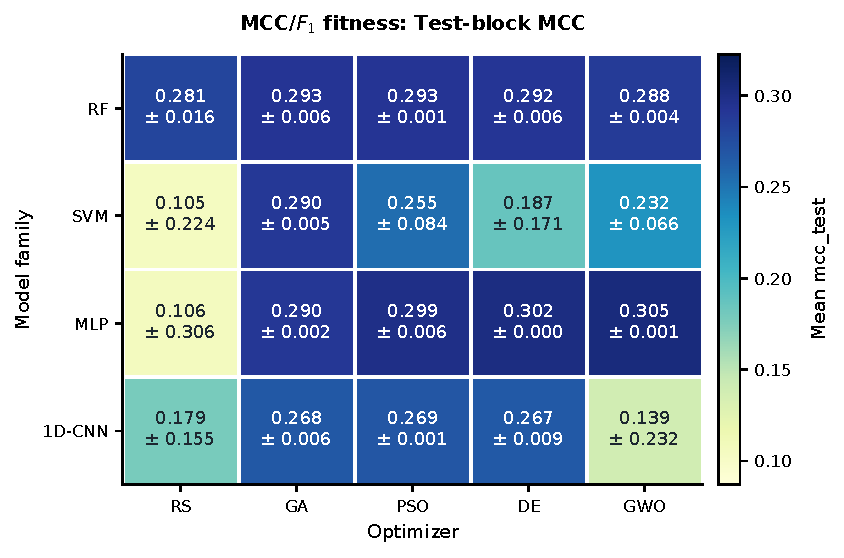
\includegraphics[width=0.95\linewidth]{figures/heatmap_mccf1_mcc_test.pdf}
\caption{Test-block MCC by classifier backbone and optimizer after selection under MCC/$F_1$ fitness. Cells report the mean and standard deviation across the three common seeds; color encodes the mean.}
\label{fig:heatmap_mccf1_mcc_test}\end{figure}

\begin{figure}[!htbp]\centering
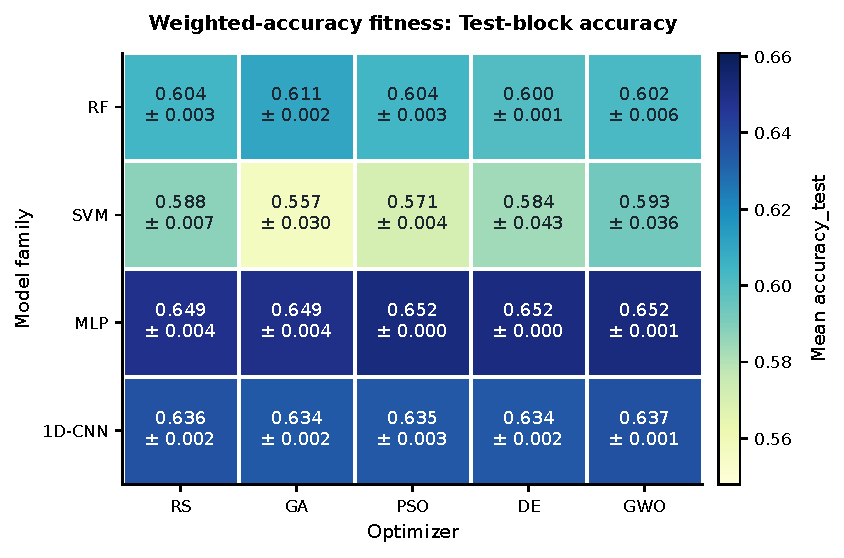
\includegraphics[width=0.95\linewidth]{figures/heatmap_accuracy_accuracy_test.pdf}
\caption{Test-block accuracy by classifier backbone and optimizer after selection under weighted-accuracy fitness. Cells report the mean and standard deviation across the three common seeds; color encodes the mean.}
\label{fig:heatmap_accuracy_accuracy_test}\end{figure}


\begin{figure}[!htbp]\centering
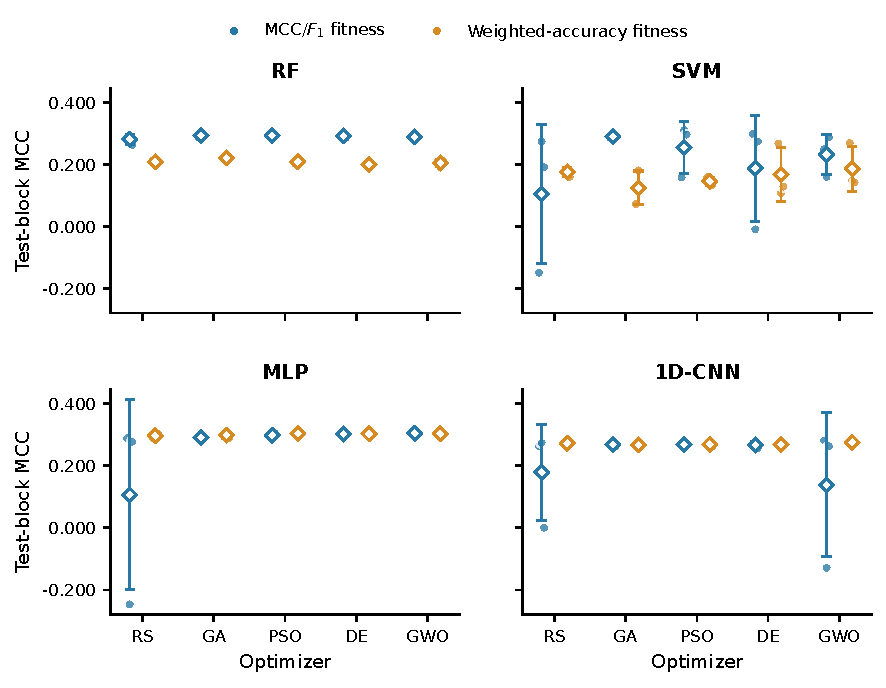
\includegraphics[width=0.90\linewidth]{figures/test_mcc_seed_points.pdf}
\caption{Test-block MCC by optimizer and backbone under MCC/$F_1$ and weighted-accuracy fitness. Facets show the four backbones; points are the three common seed-level outcomes, and diamonds with vertical bars show the mean and one standard deviation. With three observations per cell, the display is descriptive rather than inferential.}
\label{fig:test_mcc_seed_distribution}\end{figure}

\begin{figure}[!htbp]\centering
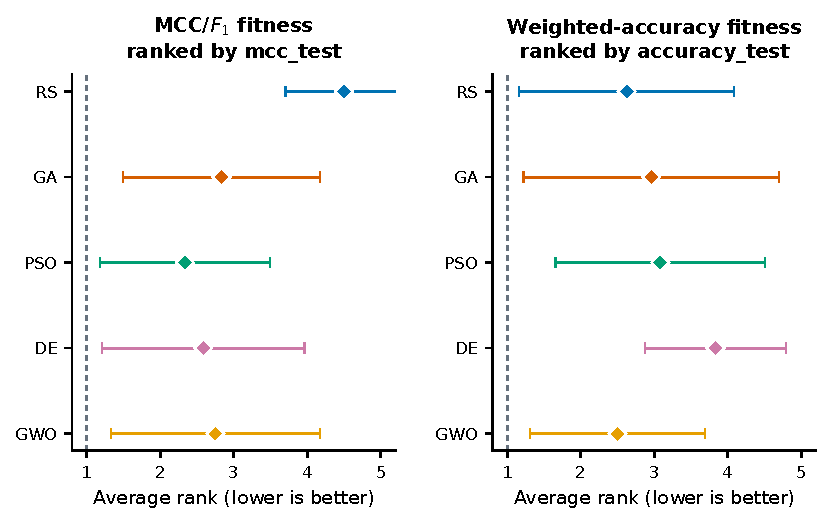
\includegraphics[width=0.90\linewidth]{figures/optimizer_average_ranks.pdf}
\caption{Descriptive average ranks of the five optimizers across 12 backbone--seed combinations (four backbones and three common seeds). Rankings use test-block MCC under MCC/$F_1$ fitness and test-block accuracy under weighted-accuracy fitness. Error bars show one standard deviation of block-level ranks; lower ranks indicate better ordering. This plot is descriptive and does not represent an optimizer significance test.}
\label{fig:optimizer_average_ranks}\end{figure}

Figure~\ref{fig:benchmark_radar} provides a normalized, multi-metric overview and is included only as a secondary summary because normalization removes the metrics' original units.



\begin{figure}[!htbp]\centering
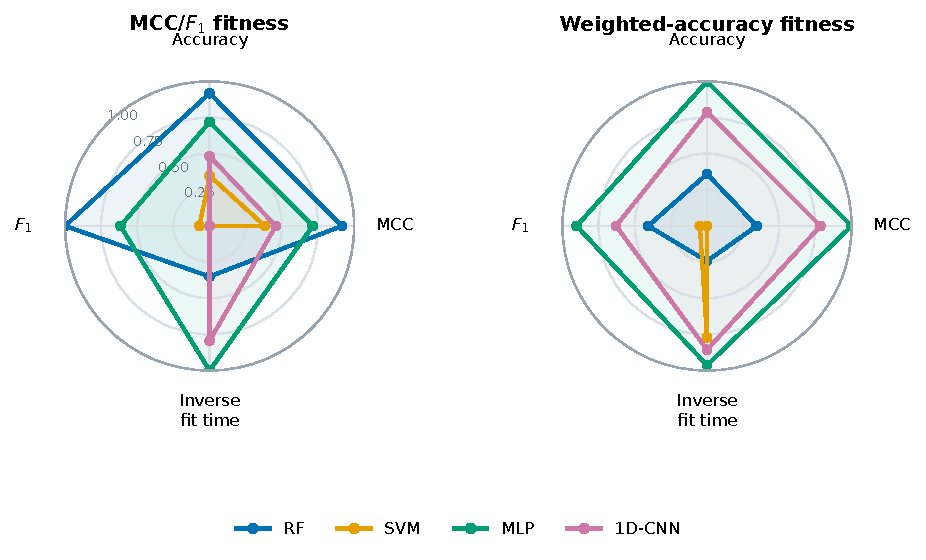
\includegraphics[width=0.95\linewidth]{figures/radar_overview_normalized.pdf}
\caption{Complementary normalized overview of test-block MCC, accuracy, $F_1$, and inverse candidate-fit time by backbone and validation objective. Values are min--max normalized across the eight backbone--protocol averages; higher values indicate better values on each axis. Candidate-fit time is log-transformed before inversion and normalization.}
\label{fig:benchmark_radar}\end{figure}

The MCC/$F_1$ panels show that extra recorded fit time is not consistently accompanied by higher test-block MCC: RF's optimizer means are tightly grouped despite differences in fit time, while SVM and MLP show optimizer-dependent score and seed-spread patterns. Under weighted-accuracy fitness, MLP and 1D-CNN occupy narrow accuracy ranges even where their fit-time positions differ; SVM shows a wider score range, but the more costly point is not uniformly the higher-scoring one. Thus, these observations do not support a general monotonic score--cost relationship. They describe cumulative uncached candidate fitting, not full search runtime, and should not be treated as an efficiency ranking. The radar profiles also vary by protocol and metric, reinforcing that no normalized shape can replace the original-scale results in Tables~\ref{tab:predictive_summary} and~\ref{tab:economic_summary}; it is a visual overview, not additional evidence for a ranking.



\section{Discussion}\label{sec:discussion}

The purpose of this benchmark is not to replace the practical pipeline of the blinded precursor, but to determine which conclusions remain when the temporal split, optimizer budget, validation objective, and economic endpoint are made explicit. The resulting evidence separates a model's average test-block outcome, its sensitivity to the optimizer--seed block, and its simplified trading consequence. This distinction matters for intraday financial prediction, where a change in selection criterion can alter a model ranking without demonstrating a stable change in market-wide forecasting ability.

The present design preserves the precursor's technical-indicator workflow and fixed seven-feature representation, but changes the comparison unit. Rather than reporting a GA-selected configuration after randomized cross-validation, every backbone is evaluated with RS, GA, PSO, DE, and GWO under the same 1,000-candidate allowance and the same chronological train/validation/test partition. Random Search is therefore a budget-matched reference against which directed population methods can be interpreted \cite{bergstra2012random_search}. The test features themselves are not used during candidate selection. However, because the target is shifted by one retained row, one training target crosses into validation and two validation targets cross into the nominal test interval. The test is therefore nominally subsequent but not strictly isolated at these three labels, and conclusions are interpreted as exploratory pending a purged rerun.

This control improves internal comparability, but it narrows the claim that the data can support. The evidence concerns four classifier families on one five-minute WIN period, conditional on an inherited input representation. It does not show that the seven indicators would be selected again in another training period, nor that an optimizer with a favourable result here will retain that advantage under another market regime. The contribution is consequently a controlled experimental frame, not a universal ordering of metaheuristics.


The test-block summaries in Table~\ref{tab:predictive_summary} show a clear reversal at the model level. Under MCC/$F_1$ fitness, RF has the largest marginal means for accuracy, MCC, and $F_1$, and its small standard deviations indicate comparatively low sensitivity to the evaluated optimizer--seed blocks. Under weighted-accuracy fitness, MLP is first on all three reported predictive measures, while 1D-CNN is also stable but remains below MLP in mean accuracy and MCC. The change in ordering is descriptive. Because the two protocols differ in both the selection metric and the inclusion of in-sample training accuracy, it cannot be attributed to metric choice alone.

MCC is useful because it summarizes the association between predicted and observed binary classes beyond raw accuracy \cite{chicco2020mcc}; however, optimizing an imbalance-aware criterion cannot guarantee the best outcome for every backbone and search trajectory. Conversely, the MLP advantage under weighted-accuracy fitness is concentrated in a low-variance regime, whereas MLP, SVM, and 1D-CNN outcomes under MCC/$F_1$ fitness vary much more across the evaluated blocks. A reported mean must therefore be accompanied by its dispersion and by the selection rule that generated it.

The rank analysis reinforces this caution. Under MCC/$F_1$ fitness, RF has the highest marginal mean MCC, but MLP has the lowest mean Friedman rank (1.533) across the matched blocks. This is not a contradiction: means weight score magnitude, whereas ranks summarize ordering within each block. Under weighted-accuracy fitness, both summaries place MLP first, and its Holm-adjusted contrasts against all other backbones are significant. Because all 15 blocks share one chronological test segment, these results indicate separation within the evaluated design rather than independent replication across time.


Figures~\ref{fig:rf_convergence_mccf1}--\ref{fig:cnn_convergence_accuracy} index progress by candidate evaluations rather than by optimizer-specific generation counts. Each line shows the mean trajectory over the three common seeds; variability envelopes are omitted to keep closely spaced optimizer curves legible. In each panel, the main y-axis is tightly bounded by the observed range of the five mean trajectories, with a small margin, and an inset magnifies the final 250 evaluations. Because limits are panel-specific, visual heights should not be compared across panels without reading their y-axis scales. Early gains indicate how quickly an optimizer locates useful regions of a search space, whereas later plateaus show the incremental benefit of additional evaluations under the fixed budget. Convergence in validation fitness does not establish equivalent generalization, so the test-block values and their dispersion in Table~\ref{tab:predictive_summary} remain necessary for interpretation.

Search behaviour interacts with the backbone and the objective. A method that improves early for RF need not be the most reliable procedure for MLP or 1D-CNN, whose mixed discrete--continuous hyperparameter spaces have different response surfaces. The article therefore does not claim a universal winner among RS, GA, PSO, DE, and GWO. A stronger optimizer-level claim would require a dedicated analysis across more seeds and temporal replications, with the optimizer itself as the inferential factor.


Table~\ref{tab:economic_summary} makes the distinction between predictive evaluation and the exploratory trading rule concrete. With next-bar execution, 1D-CNN has the largest mean net profit under both fitness protocols. Under MCC/$F_1$ fitness, RF has the least negative mean drawdown; under weighted-accuracy fitness, 1D-CNN leads mean profit, profit factor, and annualized daily Sharpe. Dispersion remains substantial for several model--protocol combinations, so the apparent return leader does not establish a stable economic advantage.

These values are reported as points under a fixed next-bar long/short rule with a five-point round-trip cost. They are not an investable-strategy claim: the evaluation does not model a full transaction-cost schedule, market impact, position sizing, or a live signal-selection policy. Its role is diagnostic: it shows that converting a one-bar-ahead regime prediction to trades can change the practical ranking of model families, and that economic reporting should accompany predictive metrics.

\subsection{Limitations and Research Agenda}

Seven limitations delimit the present evidence. First, only three seeds are common to every model--optimizer cell; standard deviations and rank tests describe the evaluated blocks, not repeated market samples. Second, exact library versions for the official TensorFlow and scikit-learn runs are not archived, and the precursor Information-Gain ranking can be traced only to the recorded seven-feature list and the researcher's recollection of a WEKA ranking on the January--March training segment; the original WEKA project, output, and settings are unavailable for independent replay. Third, the test covers one instrument and one chronological segment, so regime sensitivity and cross-market transfer remain unknown. Fourth, the Information-Gain mask was inherited from the blinded precursor rather than re-estimated on the current training segment; all conclusions are conditional on that representation. Fifth, labels are derived from retrospective hourly pivots and shifted to the next retained row. One training target crosses into validation and two validation targets cross into the nominal test block; these three rows were not purged. Four per-ticker terminal rows also lack a next-row target and retain their contemporaneous source label. A cutoff-only rerun found no other changed training or validation labels (9,032 and 3,008 checked, respectively), but this does not remove direct boundary crossings or establish causal availability of retrospective pivot labels. Consequently, test isolation is incomplete at these boundaries, and the reported comparisons should be treated as exploratory pending a purged rerun. Sixth, equalizing the budget at 1,000 evaluations establishes fairness at one computational scale but does not characterize larger-budget behaviour or wall-clock efficiency; the fit-count figure is a hardware-independent proxy and uses a run-relative threshold. Seventh, no-tuning baselines are available only for the majority rule and default RF, so the benefit of search is not isolated for SVM, MLP, or 1D-CNN.

The next study should preserve chronological evaluation and add a preregistered common 20-seed design across multiple non-overlapping market periods. It should retain pivot-confirmation timestamps, purge boundary samples whose target regime uses observations beyond the training or validation cutoff, and rerun selection and evaluation under that purged design. It should extend the present naive and default-RF references to no-tuning baselines for every backbone; archive every candidate evaluation; report compute time; and test optimizer differences separately from model differences. Re-estimating feature selection within each training window would further distinguish the effect of representation from hyperparameter search.

\section{Conclusion}\label{sec:conclusion}

This study transforms a GA-based conference precursor into a controlled benchmark for neural intraday trend classification. It preserves the predecessor's practical insight---a compact, Information-Gain-selected technical representation can support metaheuristic hyperparameter search---but replaces randomized validation and a single-optimizer design with two primary chronological holdout protocols, a separate exploratory temporal cross-validation analysis, five budget-matched optimizers, and predictive and economic assessment. The five-minute feature vector at bar $t$ is paired with the regime label at $t+1$, derived from an hourly peak-and-trough sequence detected on resampled five-minute price data.

The current evidence indicates configuration-dependent changes between the two primary fitness protocols, which differ in both metric and train/validation composition. MLP leads the predictive aggregates under weighted-accuracy fitness, while the aligned next-bar replay gives 1D-CNN the largest mean net profit under both protocols; RF has the least negative mean drawdown under MCC/$F_1$ fitness. These results reinforce the central methodological lesson: selection objective, reported metric, and economic utility must be treated as related but distinct quantities.

The manuscript deliberately avoids a confirmatory claim about a universal best fitness function because only three paired seeds are available across every cell. The hourly pivot labels are retrospective. One training target crosses into validation, two validation targets cross into the nominal test interval, four per-ticker terminal rows lack a next-row target, and the temporal-CV folds were not purged for the one-row shift. A purged rerun is needed before claiming full test isolation; multiple market periods and more seeds are also needed before stronger generalization claims. The present benchmark is exploratory evidence for this fixed chronological interval.

\FloatBarrier
% ============================================================
% Declarations
% Mirror: Al Bannoud et al. (NCA 2026) Declarations section
% ============================================================

\section*{Declarations}

\subsection*{Funding}
Funding information is withheld during double-blind review and will be supplied in the title page after editorial decision.

\subsection*{Conflict of Interest}
The authors declare that they have no conflict of interest or competing financial interests.

\subsection*{Ethical Approval}
This article does not contain any studies with human participants or animals performed by any of the authors.

\subsection*{Data and Code Availability}
The datasets generated and analyzed during the current study, along with the complete source code for all optimization algorithms, benchmark scripts, and evaluation pipelines, are available in the project repository upon reasonable request.

\subsection*{Author Contributions}
Author-contribution information is withheld during double-blind review and will be supplied in the title page after editorial decision.


% Keep each reference together and tighten list spacing to avoid isolated lines at page breaks.
{\interlinepenalty=10000\relax
 \setlength{\bibsep}{0.5em}%
 \bibliography{references}}
\end{document}
